\addtocontents{toc}{\protect\newpage}
\chapter{Робота з документами}

\section{Вхідний документ}

\subsection{Реєстрація}

Для Реєстрації документа:

--- Натисніть на кнопку «Новий документ» (виділено червоною рамкою на Рисунку 5.1.1.1)

\begin{figure}[!htbp]
\centerline{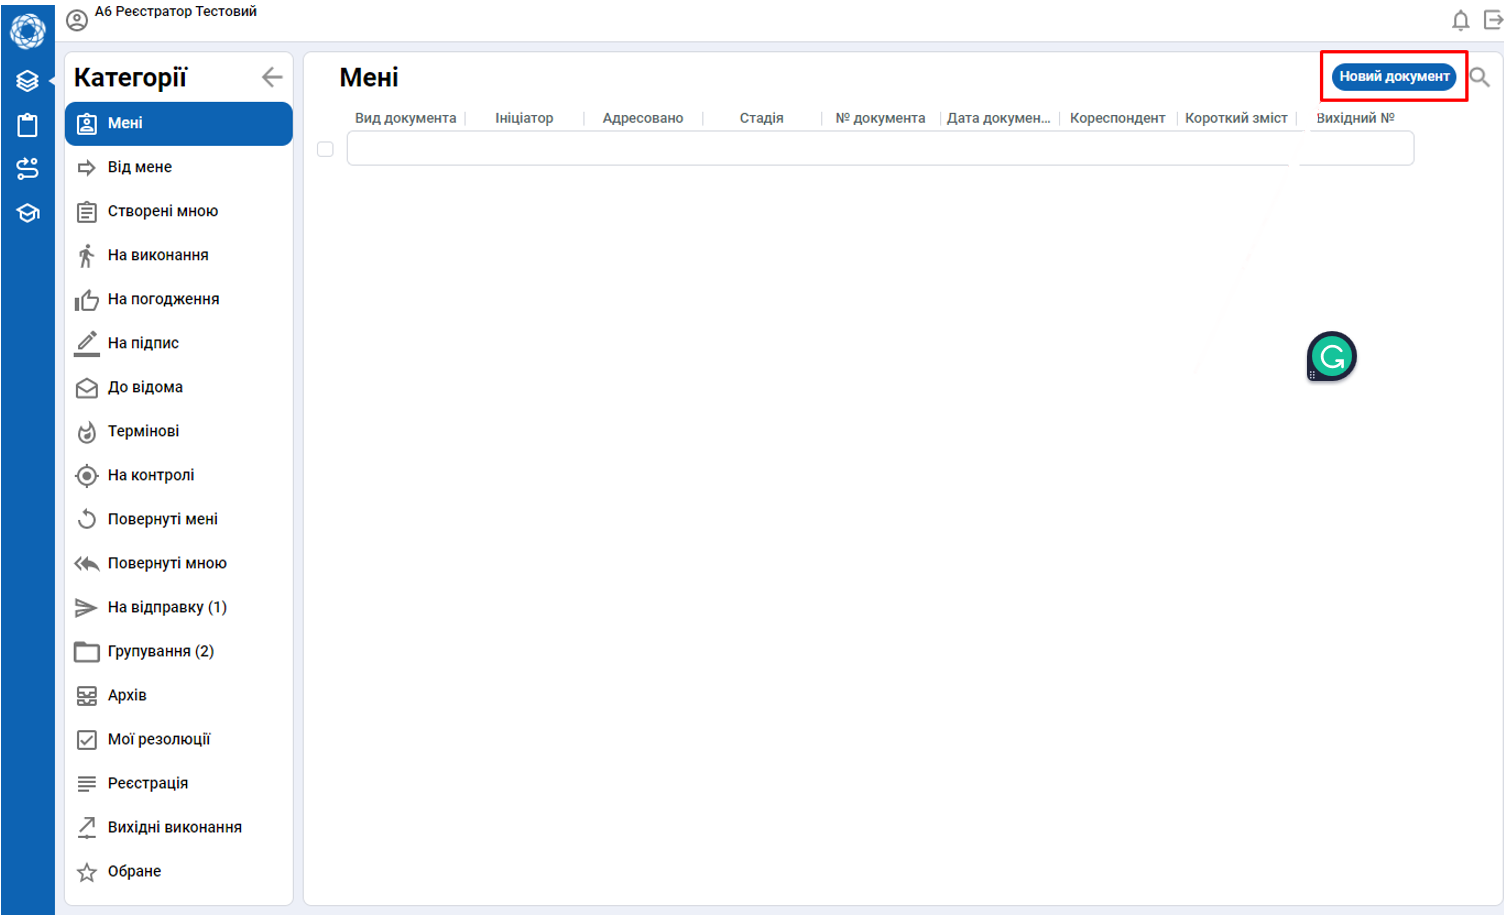
\includegraphics[width=\textwidth]{img/5.1.1.1.png}}
\caption{Рис. 5.1.1.1. Створення нового документа}
\end{figure}

--- Оберіть вид документа з переліку --- Вхідний документ (див. Рисунок 5.1.1.2)

\begin{figure}[!htbp]
\centerline{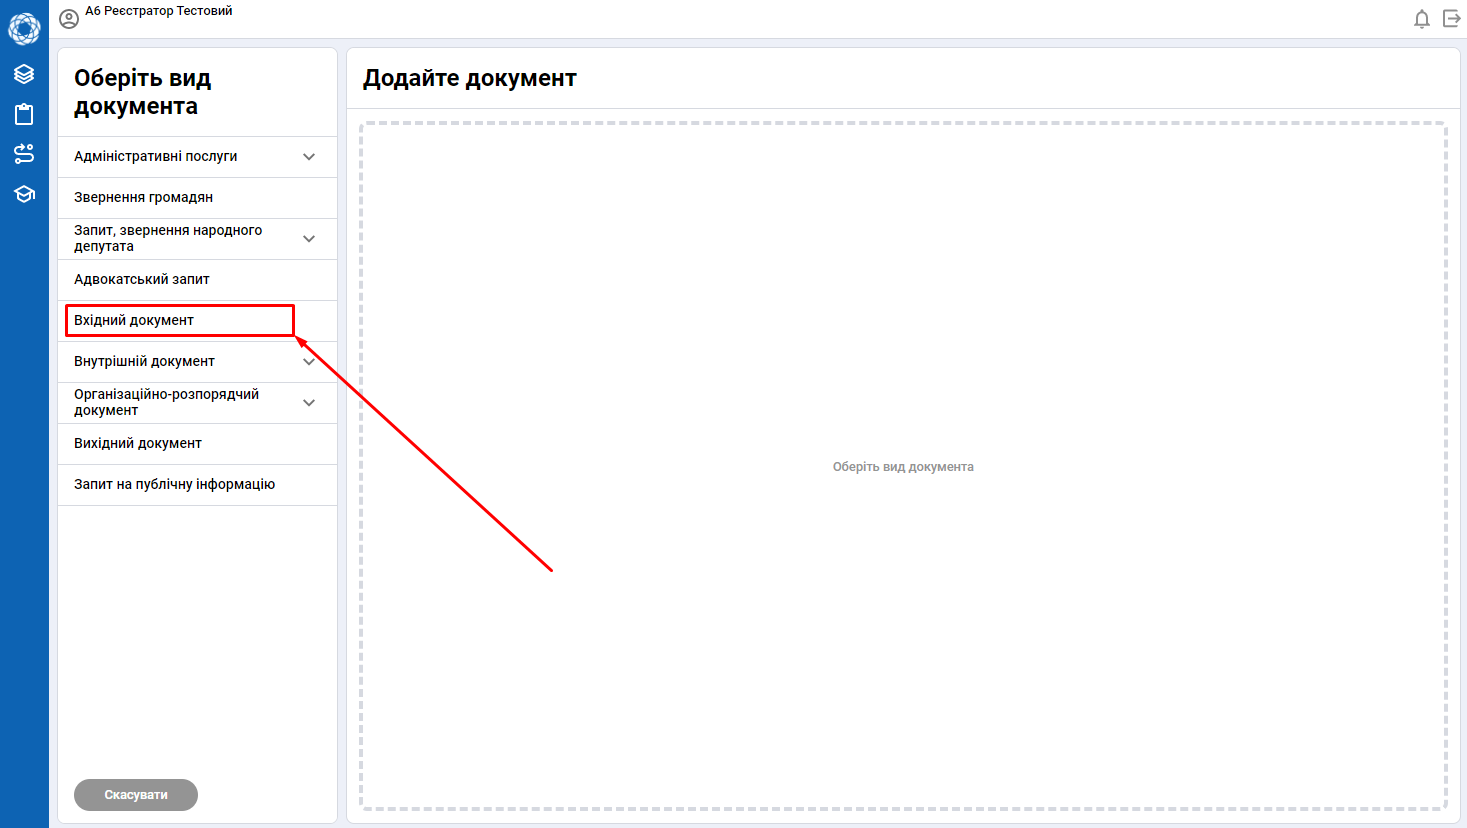
\includegraphics[width=\textwidth]{img/5.1.1.2.png}}
\caption{Рис. 5.1.1.2. Вибір виду документа}
\end{figure}

--- Заповніть РМК (область введення інформації позначена цифрою \circled{3} на
Рисунку 5.1.1.3 \circled{$\ast$} --- поле обов'язкове для заповнення)

\begin{figure}[!htbp]
\centerline{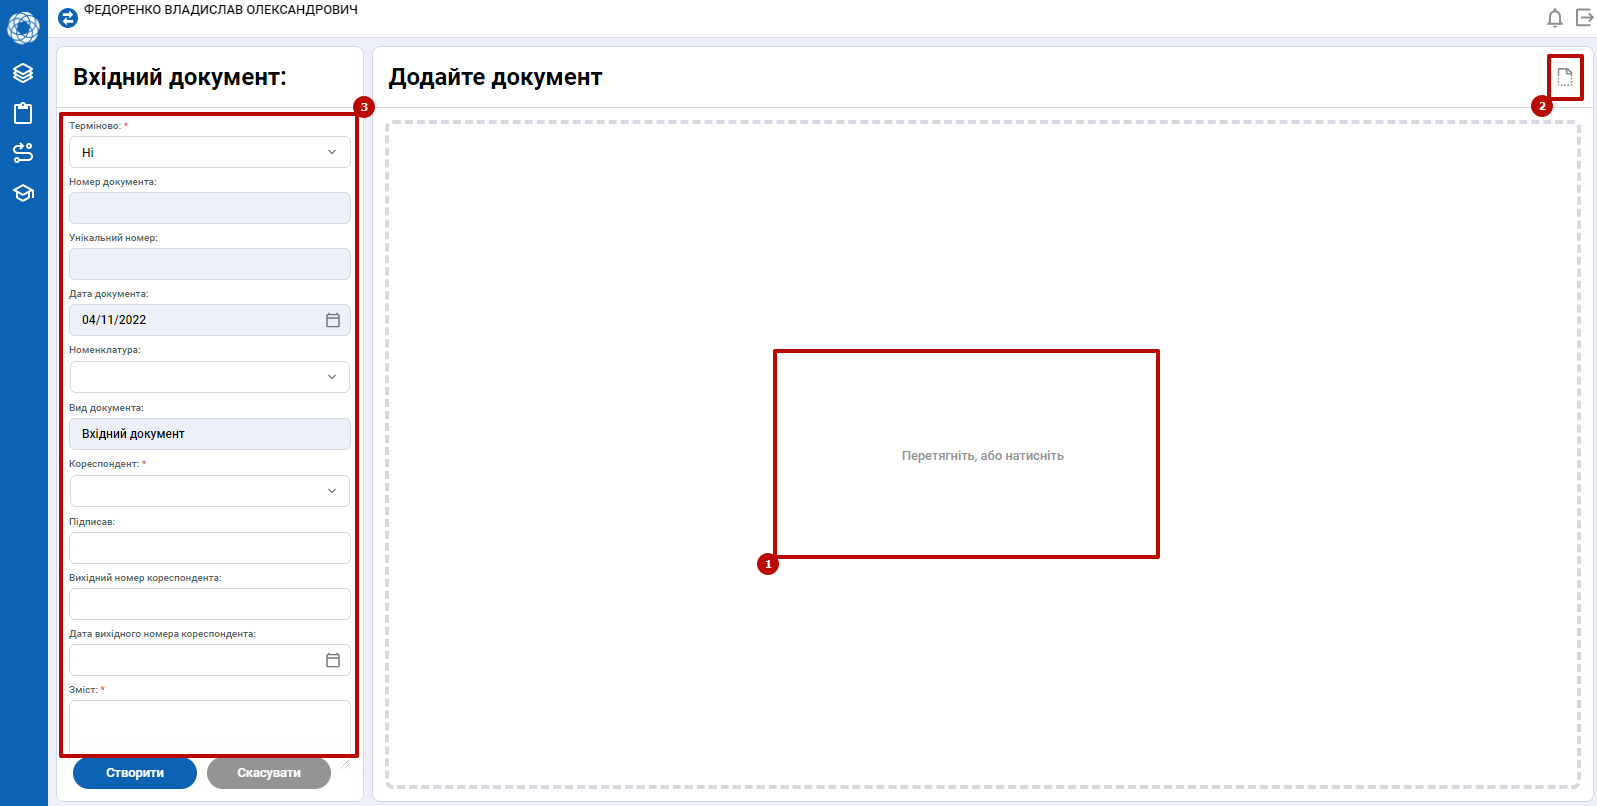
\includegraphics[width=\textwidth]{img/5.1.1.3.png}}
\caption{Рис. 5.1.1.3. Створення РМК}
\end{figure}

--- Додайте файл вхідного документа у зручний для Вас спосіб:
1) активний елемент «Перетягніть, або натисніть», позначений цифрою 1 на Рисунку 5.1.1.3;
2) шляхом сканування $\rightarrow$ піктограма 2 «Сканувати» у правому куті екранної форми (див. Рисунку 5.1.1.3).

\subsection{Сканування}

Для Сканування документа:

--- натисніть піктограму «Сканувати» → відкриється інтерфейс для процесу
сканування (див. Рисунку 5.1.2.1);

--- оберіть необхідний сканер з переліку → позначено цифрою \circled{1};

--- оберіть якість → позначено цифрою \circled{2};

--- за необхідності відредагуйте, використовуючи панель інструментів →
область редагування позначена цифрою \circled{3} в лівій частині екранної форми;

--- оберіть ім'я файлу → позначено цифрою \circled{4};

--- збережіть документ → позначено цифрою \circled{5}.

\begin{figure}[!htbp]
\centerline{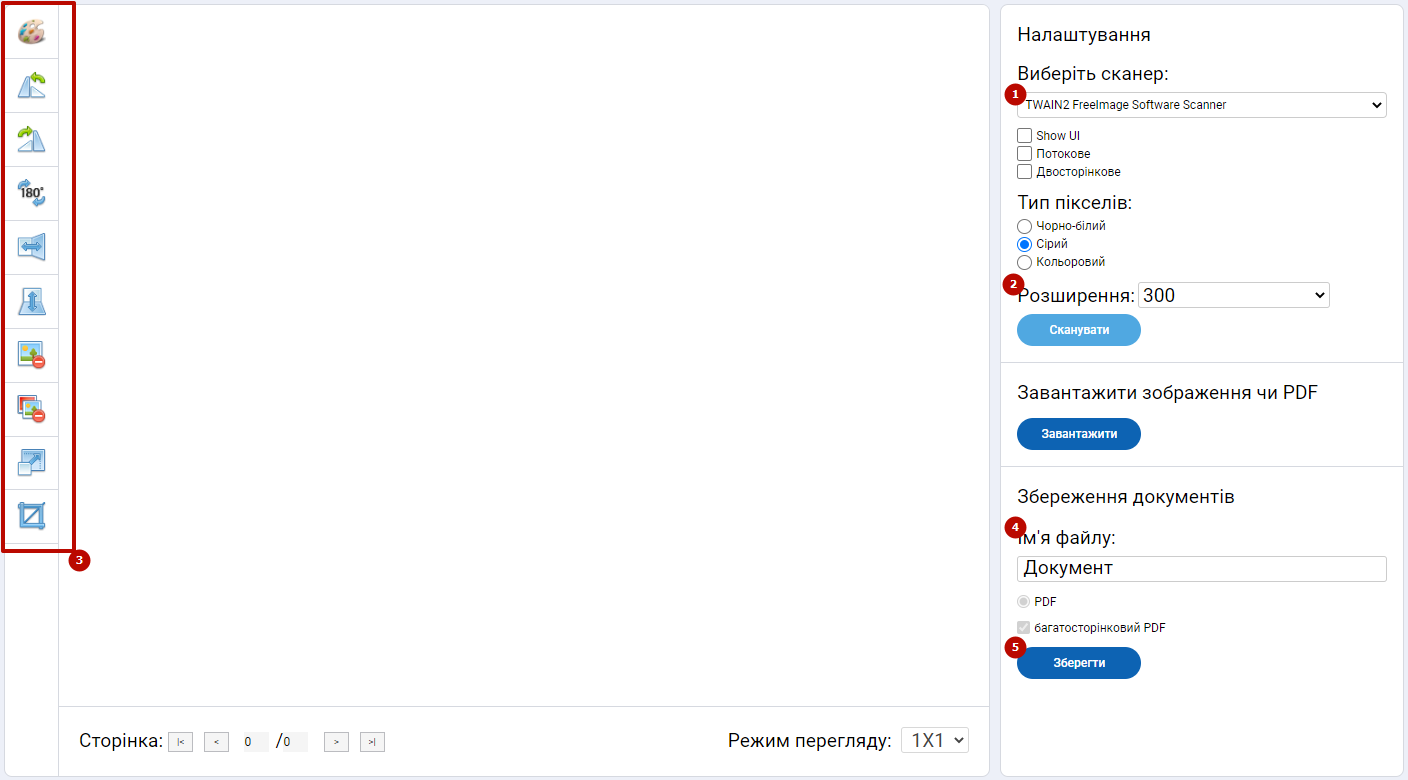
\includegraphics[width=\textwidth]{img/5.1.2.1.png}}
\caption{Рис. 5.1.2.1. Процес сканування}
\end{figure}

Доданий документ на екрані буде виглядати так, як зображено на Рисунку 5.1.2.2:

--- щоб виділити основний документ від його додатків → натисніть кнопку «Зробити основним», позначено цифрою \circled{1};

--- щоб закінчити процес створення документа → натисніть активний елемент «Створити», позначено цифрою \circled{2}.

\begin{figure}[!htbp]
\centerline{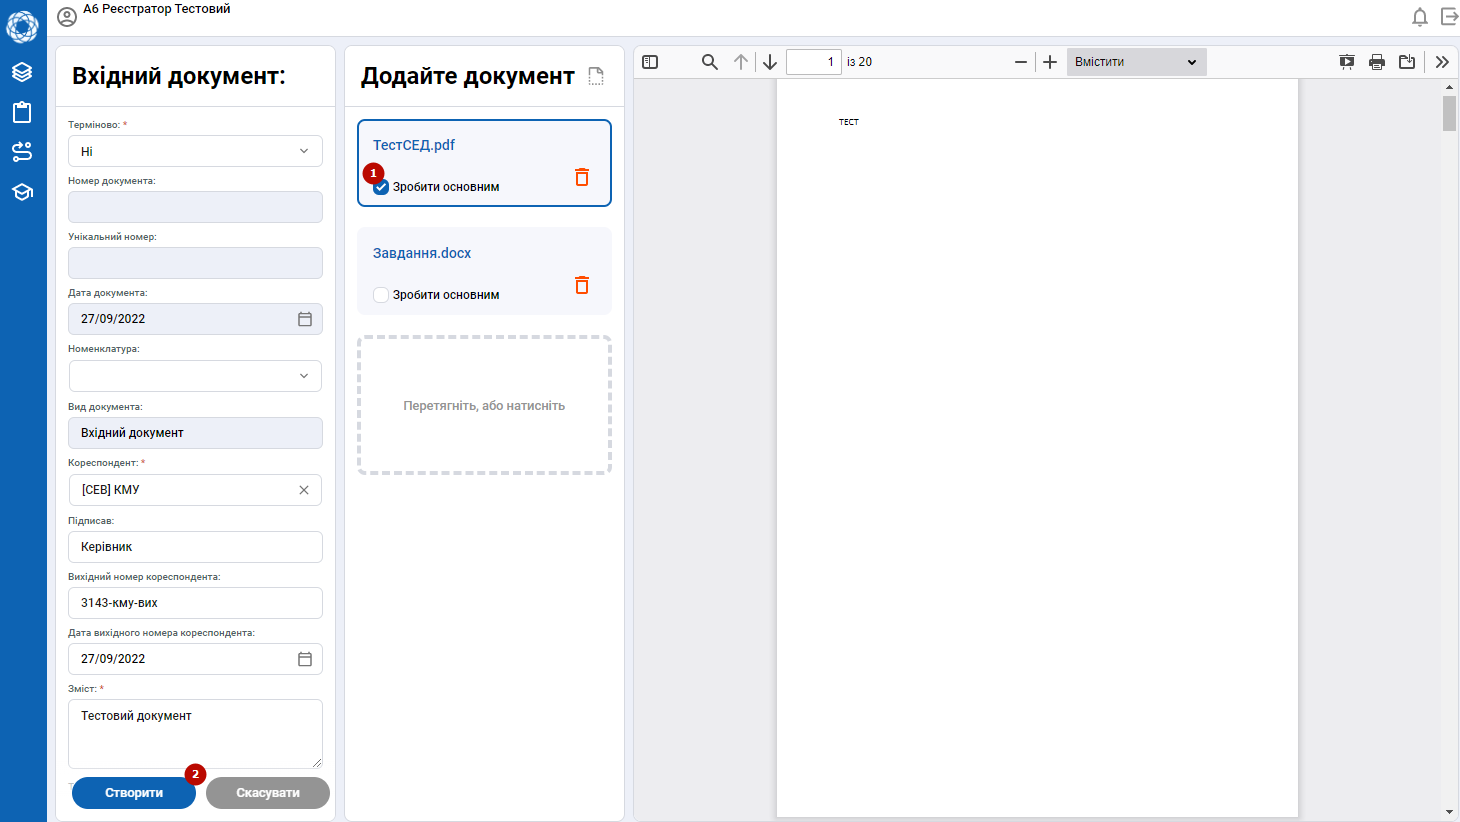
\includegraphics[width=\textwidth]{img/5.1.2.2.png}}
\caption{Рис. 5.1.2.2. Процес створення документа}
\end{figure}

\subsection{Редагування}

Для Редагування реєстраційно-моніторингової картки:

--- натисніть на піктограму із зображенням олівця у правому верхньому куті
лівої частини екранної форми, позначено цифрою \circled{1} на Рисунку 5.1.3.1;

\begin{figure}[!htbp]
\centerline{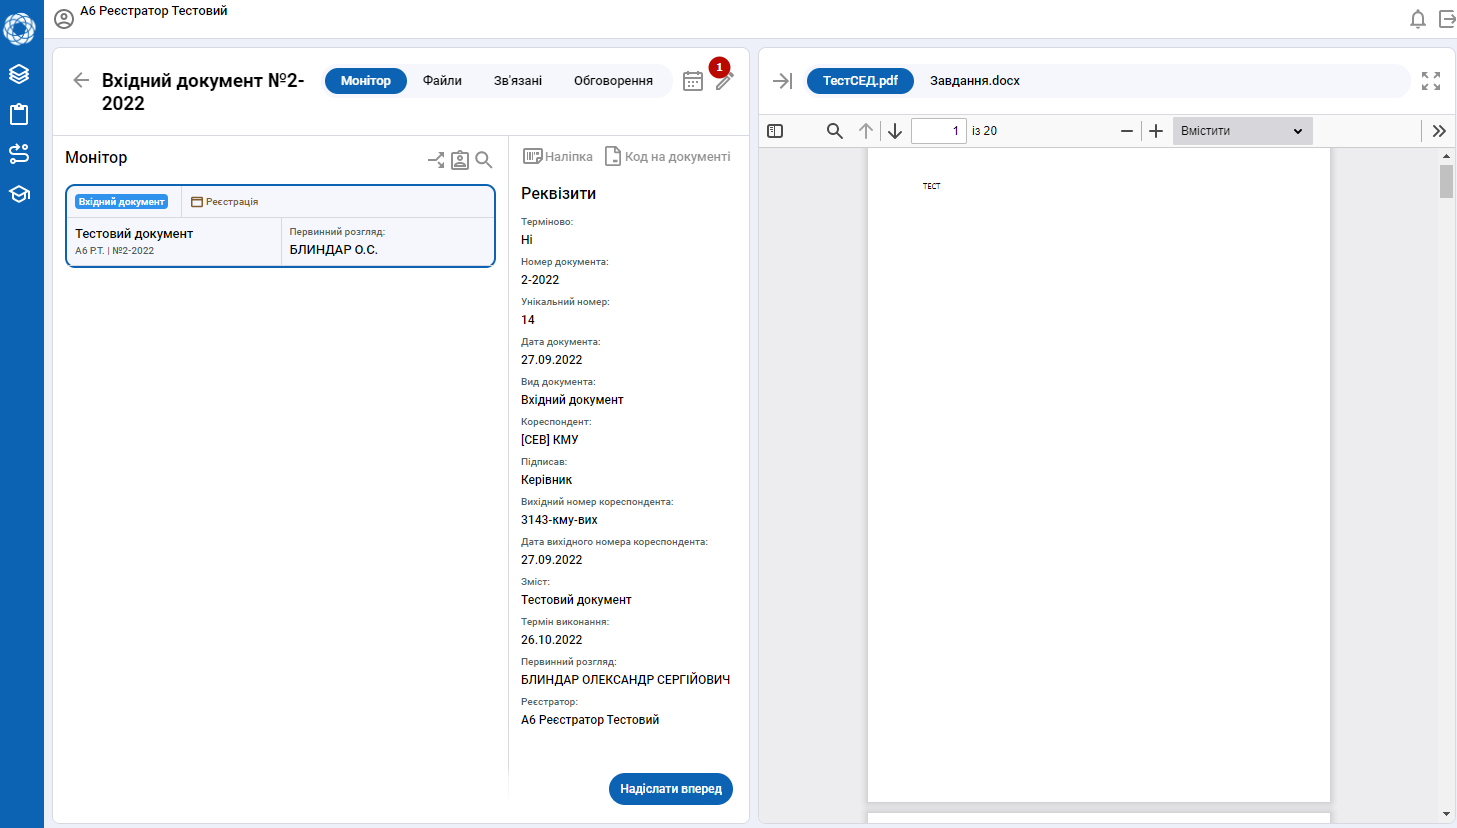
\includegraphics[width=\textwidth]{img/5.1.3.1.png}}
\caption{Рис. 5.1.3.1. Редагування}
\end{figure}

інтерфейс документа видозміниться так, як показано на Рисунку 5.1.3.2;
--- для внесення змін в документ скористайтеся активними елементами,
позначені цифрами на Рисунку 5.1.3.2: \circled{1} --- область для внесення змін реквізитів;
\circled{2} --- активний елемент, що розкриває додаткове меню, де можна додавати/
видаляти документи (див. Рисунку 5.1.3.3 підменю позначено цифрою 2.1);
\circled{3} --- можливість сканування документів.

\begin{figure}[!htbp]
\centerline{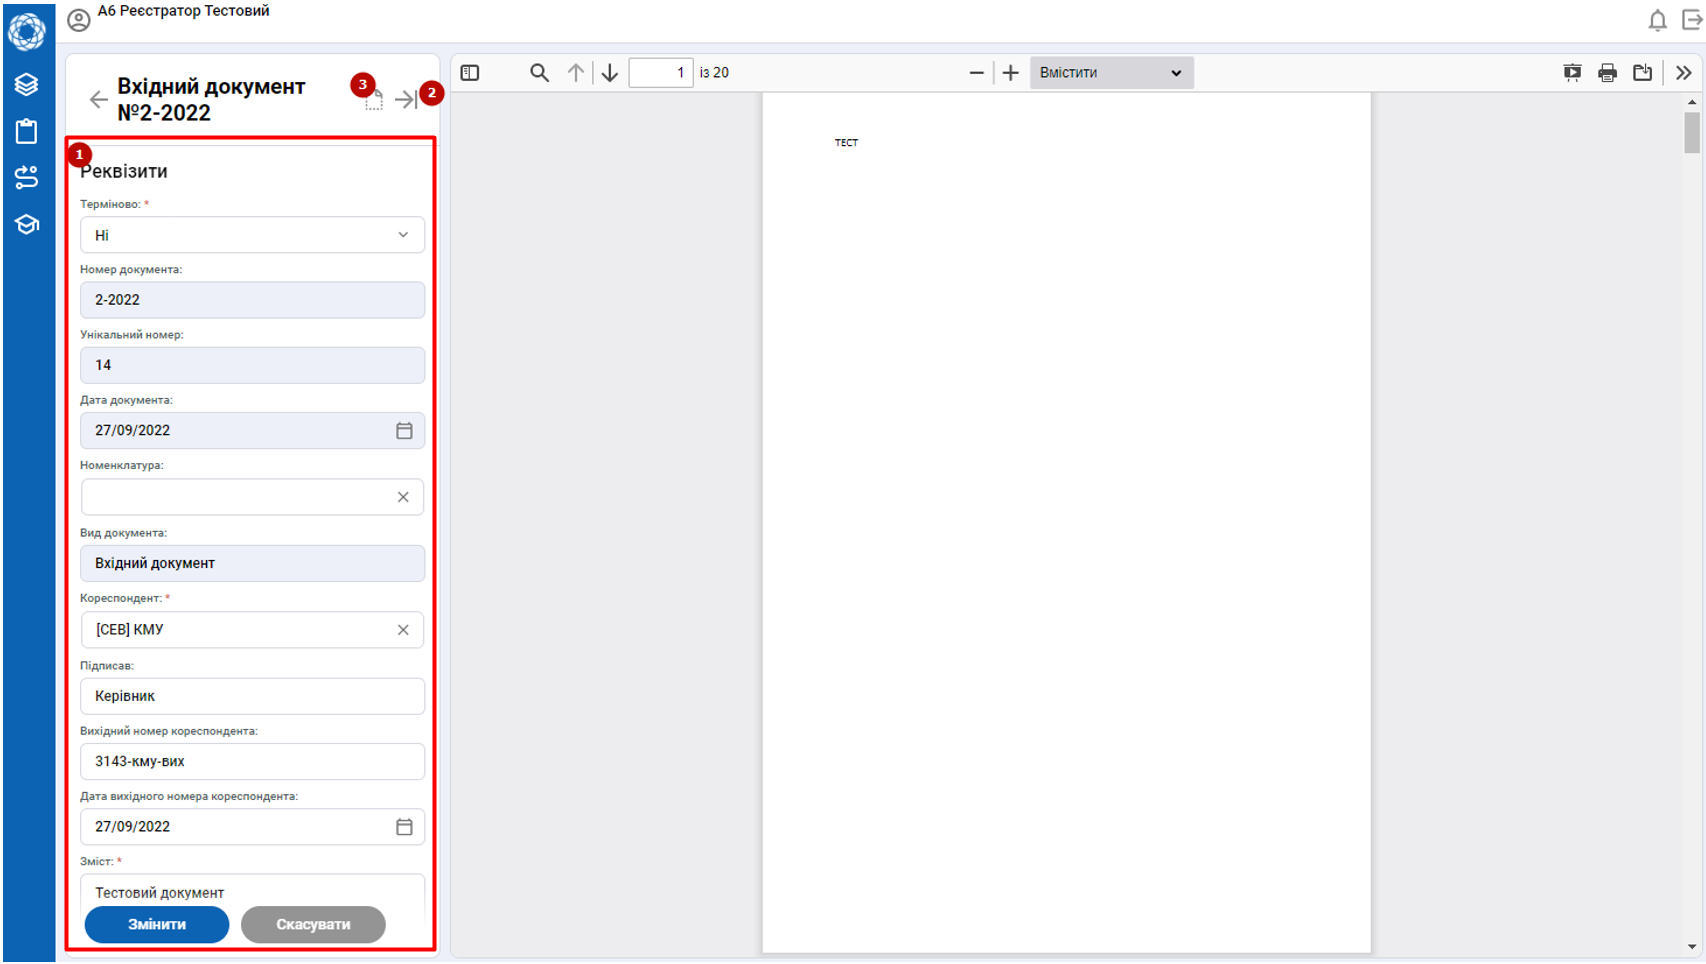
\includegraphics[width=\textwidth]{img/5.1.3.2.png}}
\caption{Рис. 5.1.3.2. Процес редагування документа}
\end{figure}

щоб додати/ видалити документ → скористайтеся активним елементом
позначеним цифрою 2 на Рисунку 5.1.3.2 → у розкритому підменю 2.1 (див.
Рисунку 5.1.3.3) виконайте необхідні дії;

--- щоб закріпити зміни → натисніть «Змінити» позначено цифрою \circled{1} або
«Скасувати» позначено цифрою \circled{2} на Рисунку 5.1.3.3.

\begin{figure}[!htbp]
\centerline{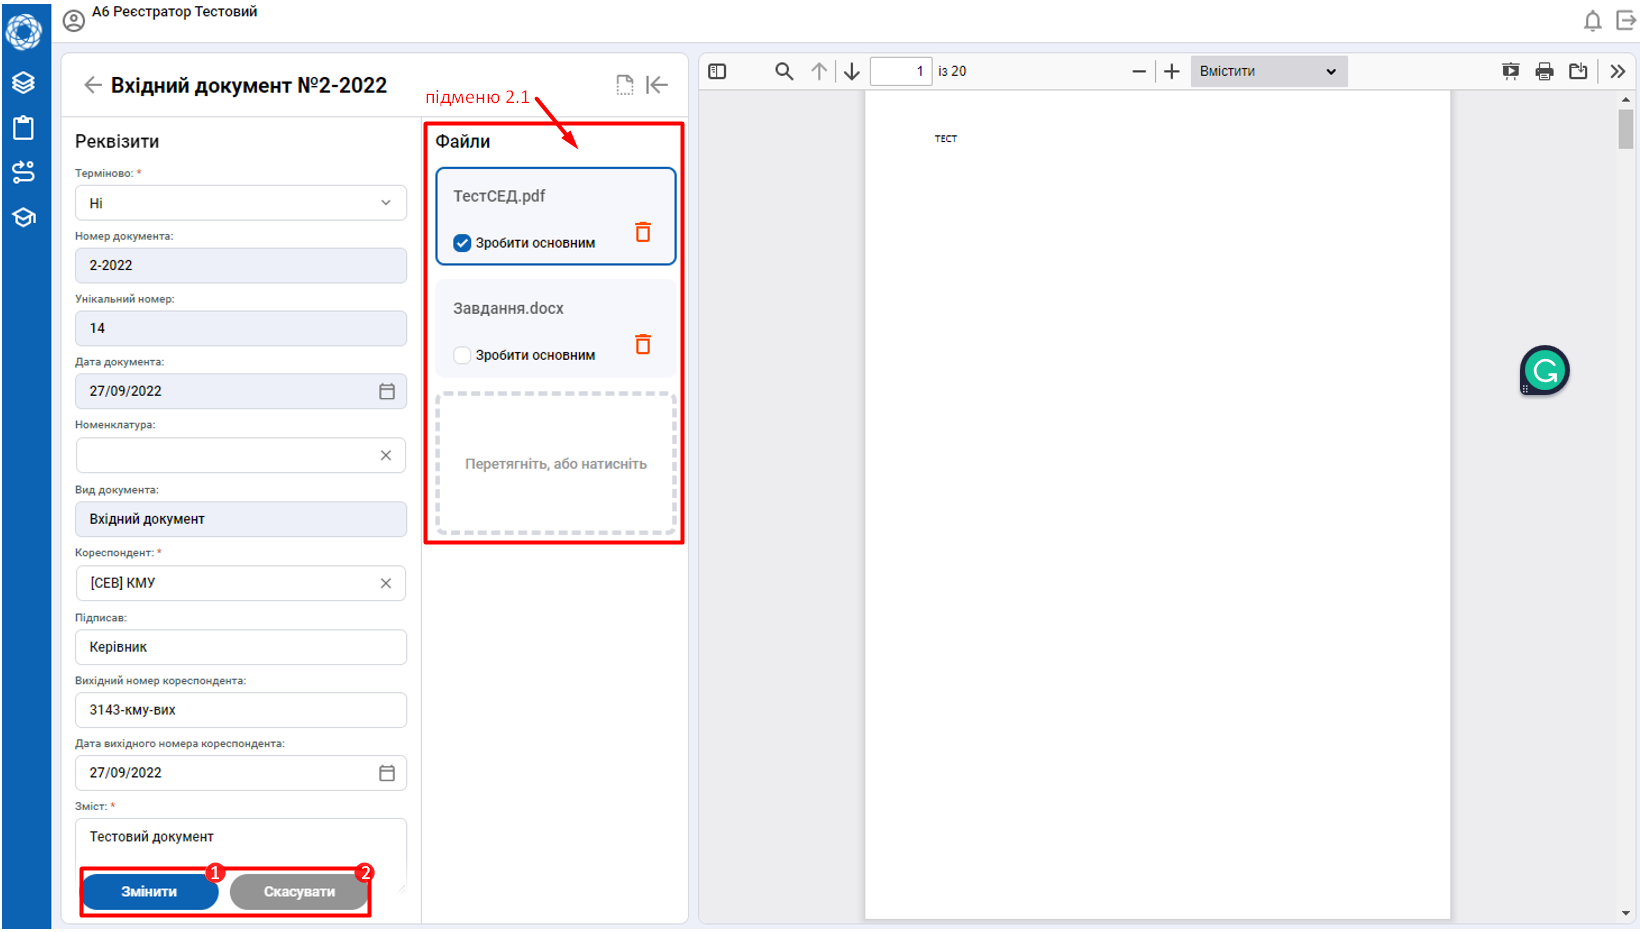
\includegraphics[width=\textwidth]{img/5.1.3.3.png}}
\caption{Рис. 5.1.3.3. Закінчення редагування документа}
\end{figure}

Для закінчення процесу Реєстрації документа:
--- натисніть активний елемент «Надіслати вперед» → позначено цифрою \circled{1} на Рисунку 5.1.3.4;
--- такі дії можливі в разі визначення особи первинного розгляду → позначено рамкою на Рисунку 5.1.3.4;

\begin{figure}[!htbp]
\centerline{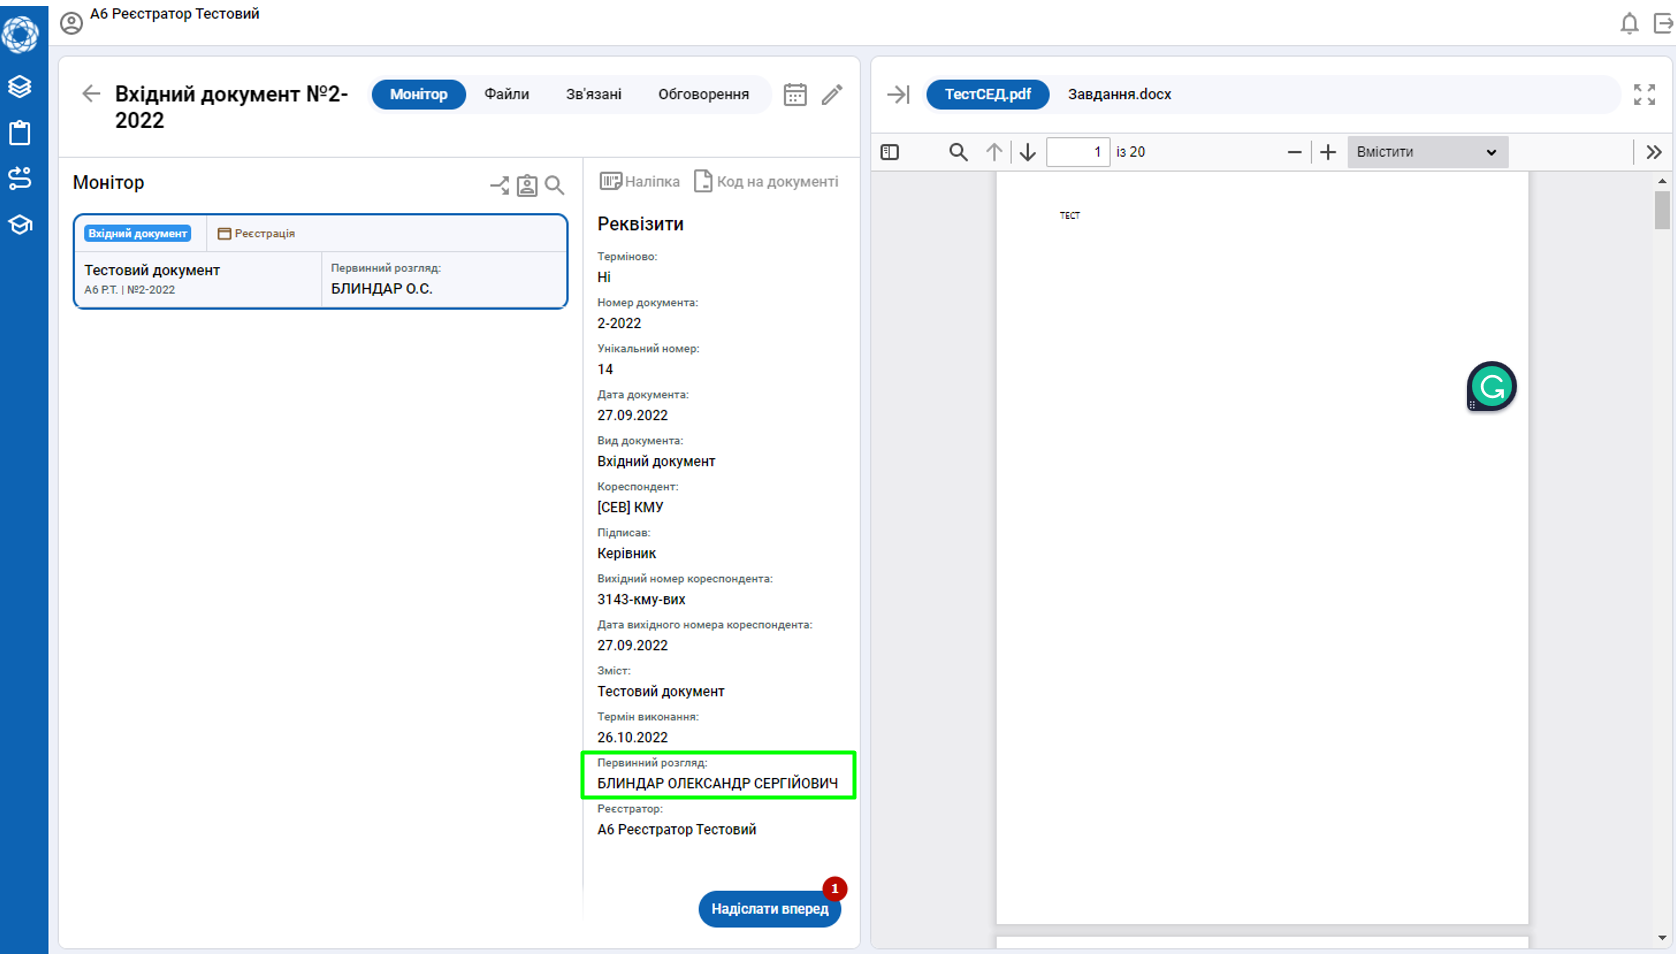
\includegraphics[width=\textwidth]{img/5.1.3.4.png}}
\caption{Рис. 5.1.3.4. Завершальний етап процесу реєстрації документа}
\end{figure}

якщо особа первинного розгляду не вказана → натиснуть активний елемент
«Надіслати вперед» → позначено цифрою \circled{1} на Рисунку 5.1.3.5 → документ
буде скеровано відповідальній особі на стадію «Визначення», яка визначить особу первинного розгляду.
--- Поруч з папкою «На визначення» з'явиться

\begin{figure}[!htbp]
\centerline{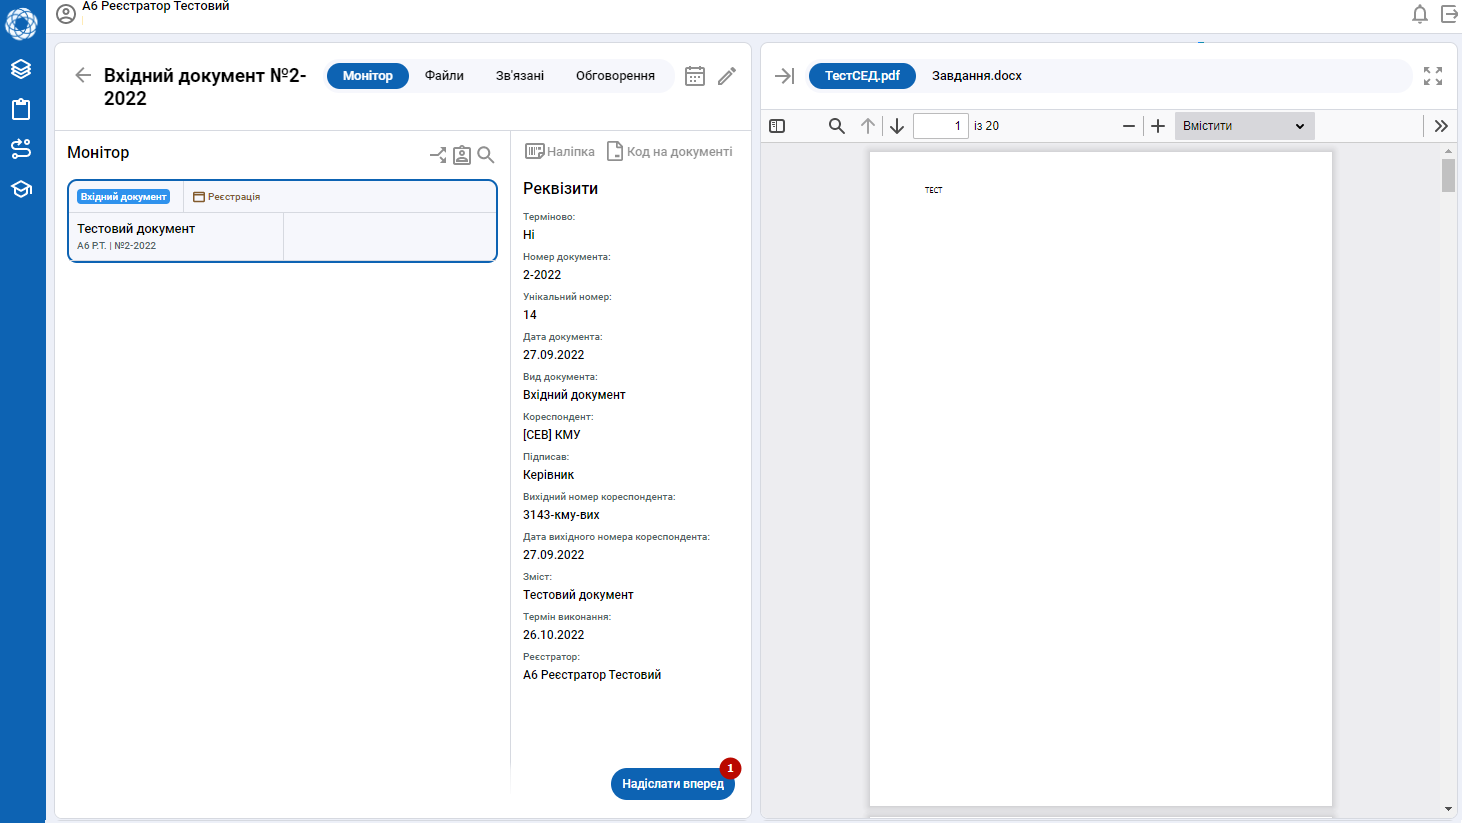
\includegraphics[width=\textwidth]{img/5.1.3.5.png}}
\caption{Рис. 5.1.3.5. Не вказано особу первинного розгляду}
\end{figure}

\subsection{Визначення}

Папка «На визначення» (див. Рисунок 5.1.4.1) містить документи, що потребують
визначення особи або декількох осіб первинного розгляду.
Особу/ осіб первинного розгляду визначає користувач, що має відповідні
повноваження (помічник директора, директор).

\begin{figure}[!htbp]
\centerline{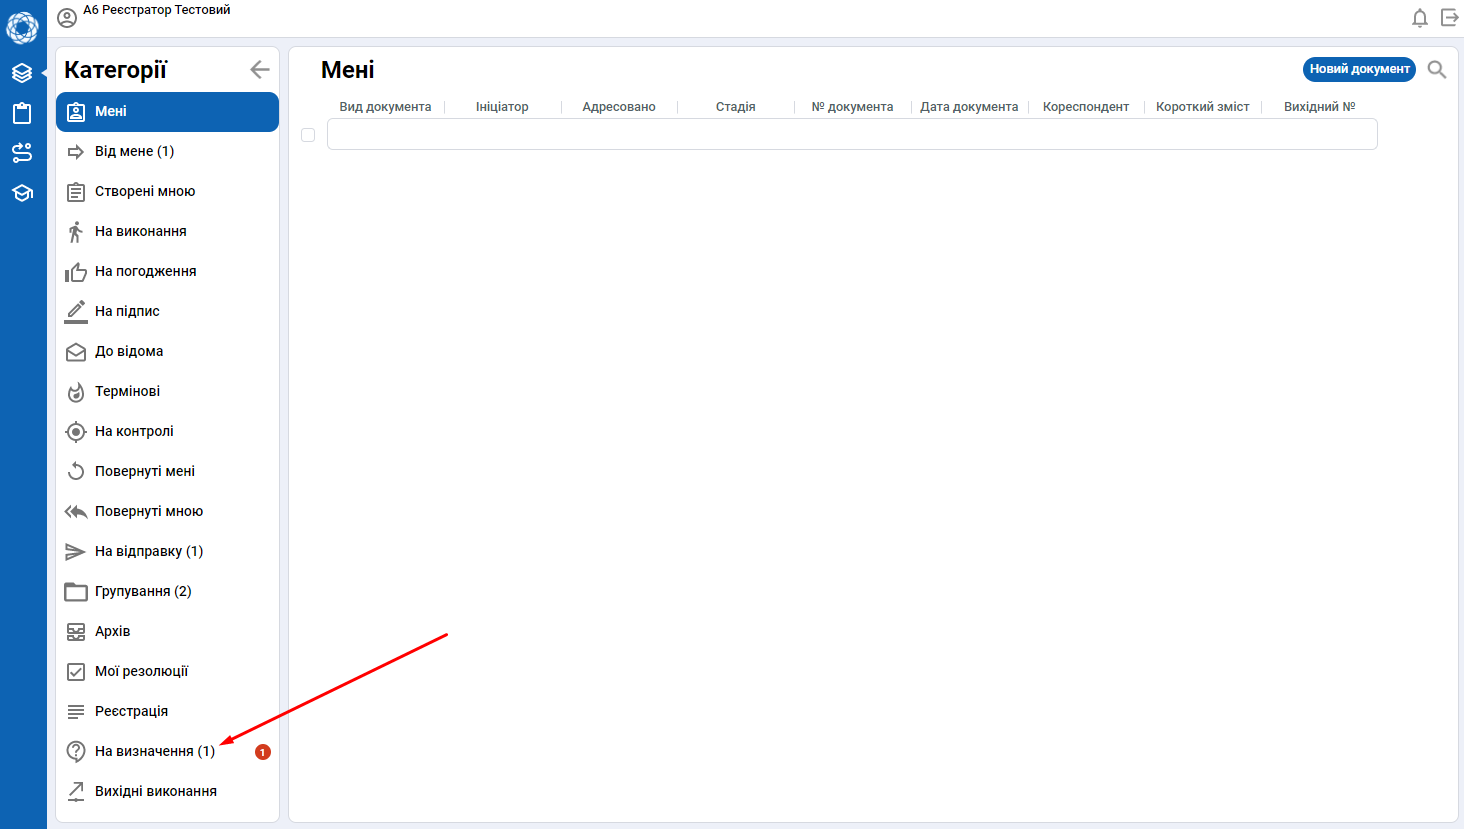
\includegraphics[width=\textwidth]{img/5.1.4.1.png}}
\caption{Рис. 5.1.4.1. Меню робочого столу користувача}
\end{figure}

Для визначення осіб первинного розгляду:
--- відкрийте документ → натисніть на піктограму із зображенням олівця
(Редагування) → позначено цифрою \circled{1} на Рисунку 5.1.4.2;

\begin{figure}[!htbp]
\centerline{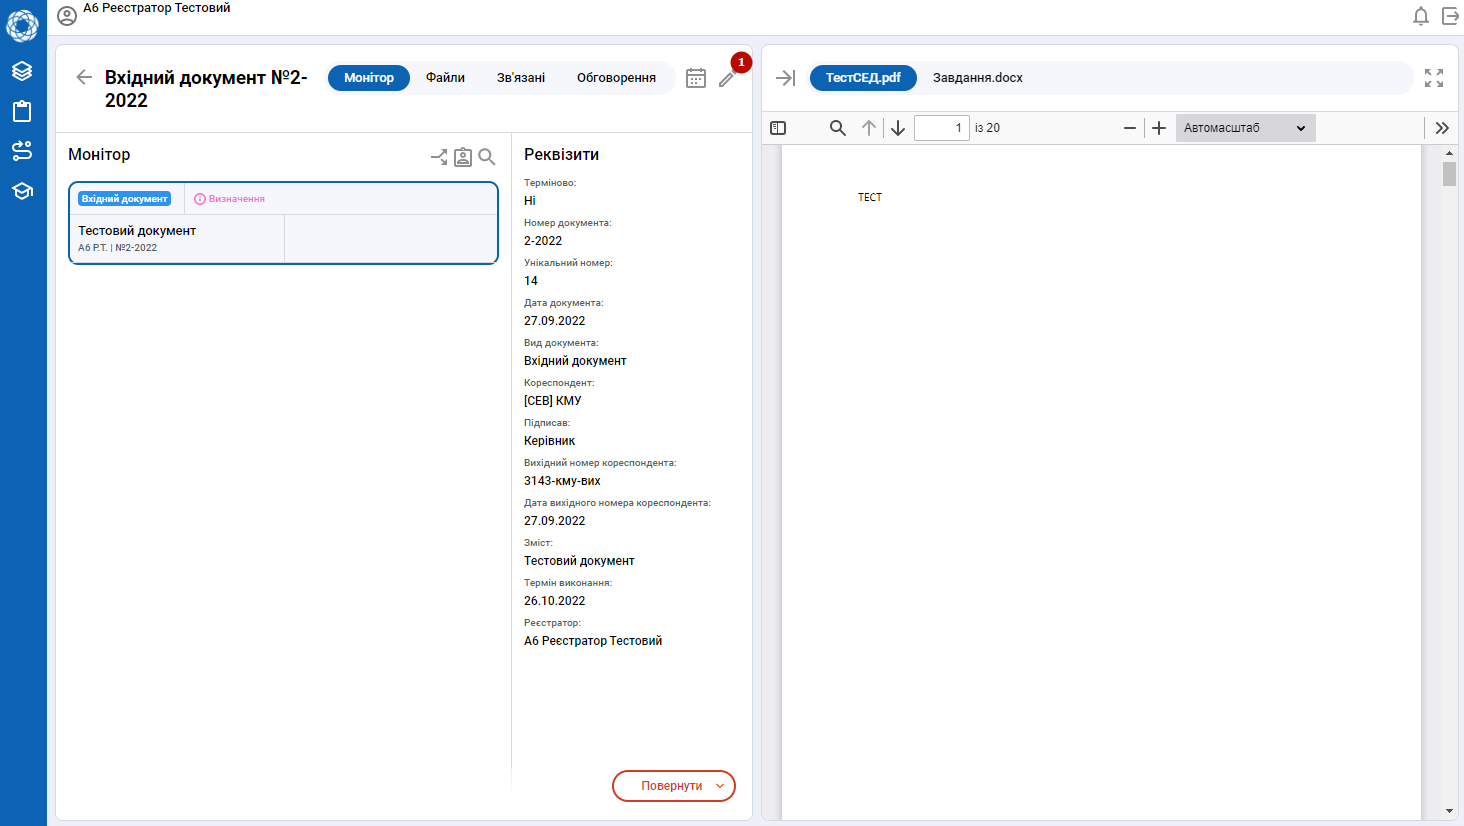
\includegraphics[width=\textwidth]{img/5.1.4.2.png}}
\caption{Рис. 5.1.4.2. }
\end{figure}

заповніть поле «Первинний розгляд» → позначено цифрою \circled{1} на Рисунку 5.1.4.3;
--- щоб підтвердити зміни → натисніть активний елемент «Змінити» → позначено цифрою \circled{2} на Рисунку 5.1.4.3.

\begin{figure}[!htbp]
\centerline{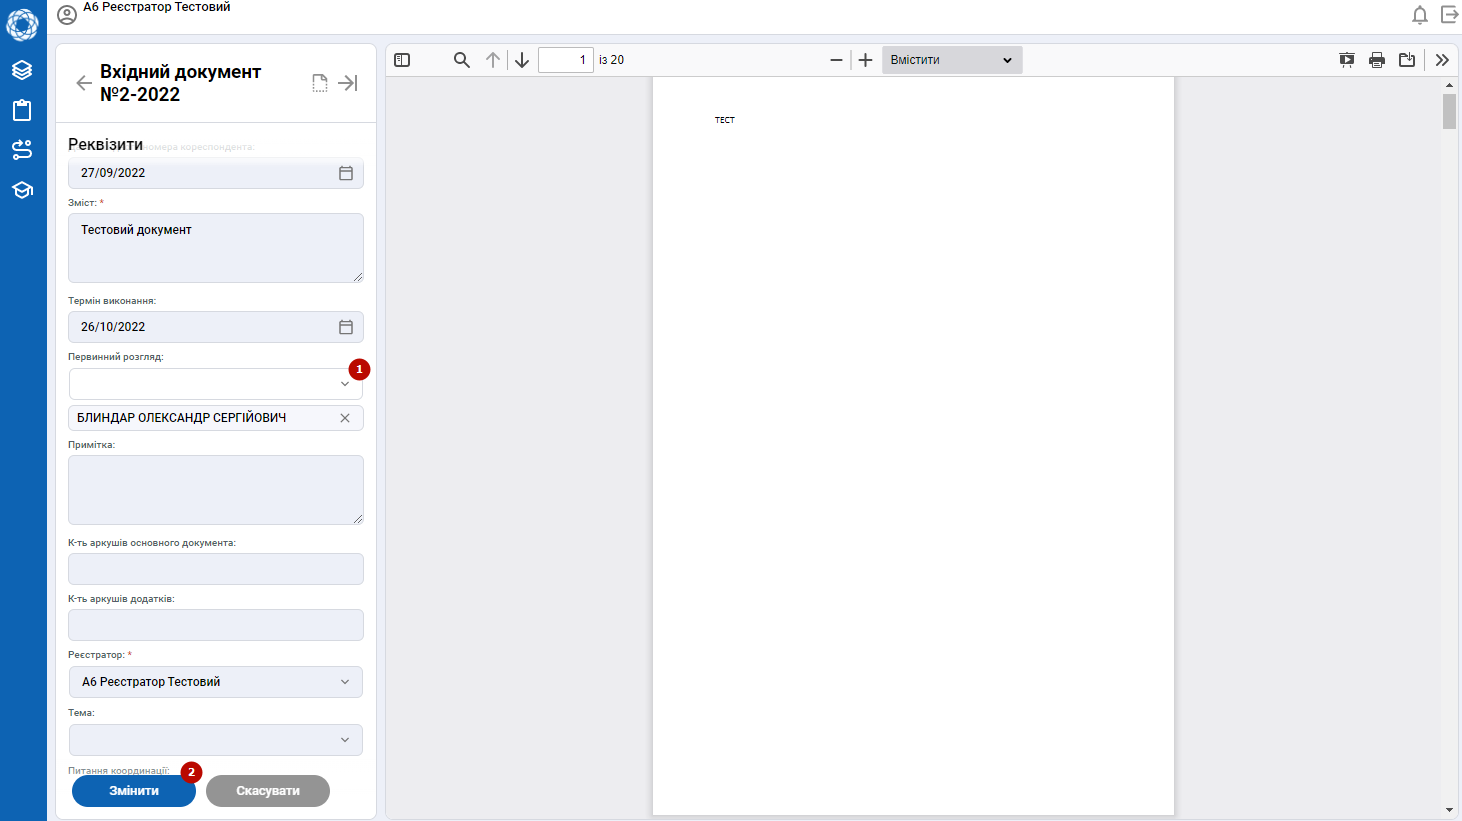
\includegraphics[width=\textwidth]{img/5.1.4.3.png}}
\caption{Рис. 5.1.4.3. }
\end{figure}

щоб завершити процес «Визначення» → натисніть активний елемент «На
первинний розгляд» → позначено цифрою \circled{1} на Рисунку 5.1.4.4.

\begin{figure}[!htbp]
\centerline{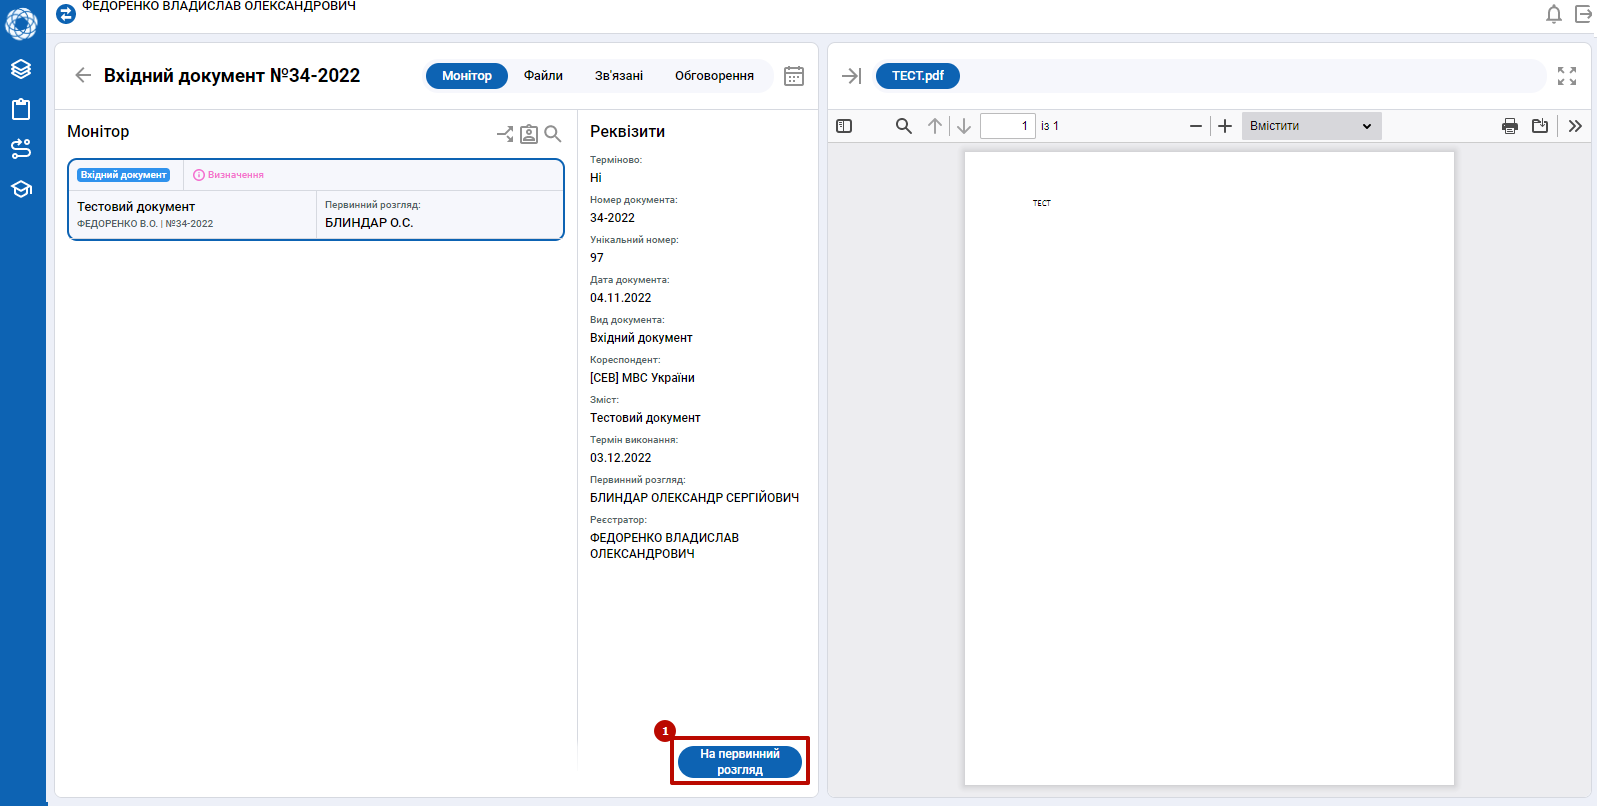
\includegraphics[width=\textwidth]{img/5.1.4.4.png}}
\caption{Рис. 5.1.4.4. }
\end{figure}

\section{Резолюція}

\subsection{Повернення документа на реєстрацію}

Для повернення вхідного документа на Реєстрацію:
--- натисніть активний елемент «Повернути» → позначено цифрою \circled{1} на Рисунку 5.2.1.1;
--- виберіть пункт «На реєстрацію» → позначено цифрою \circled{2}.

\begin{figure}[!htbp]
\centerline{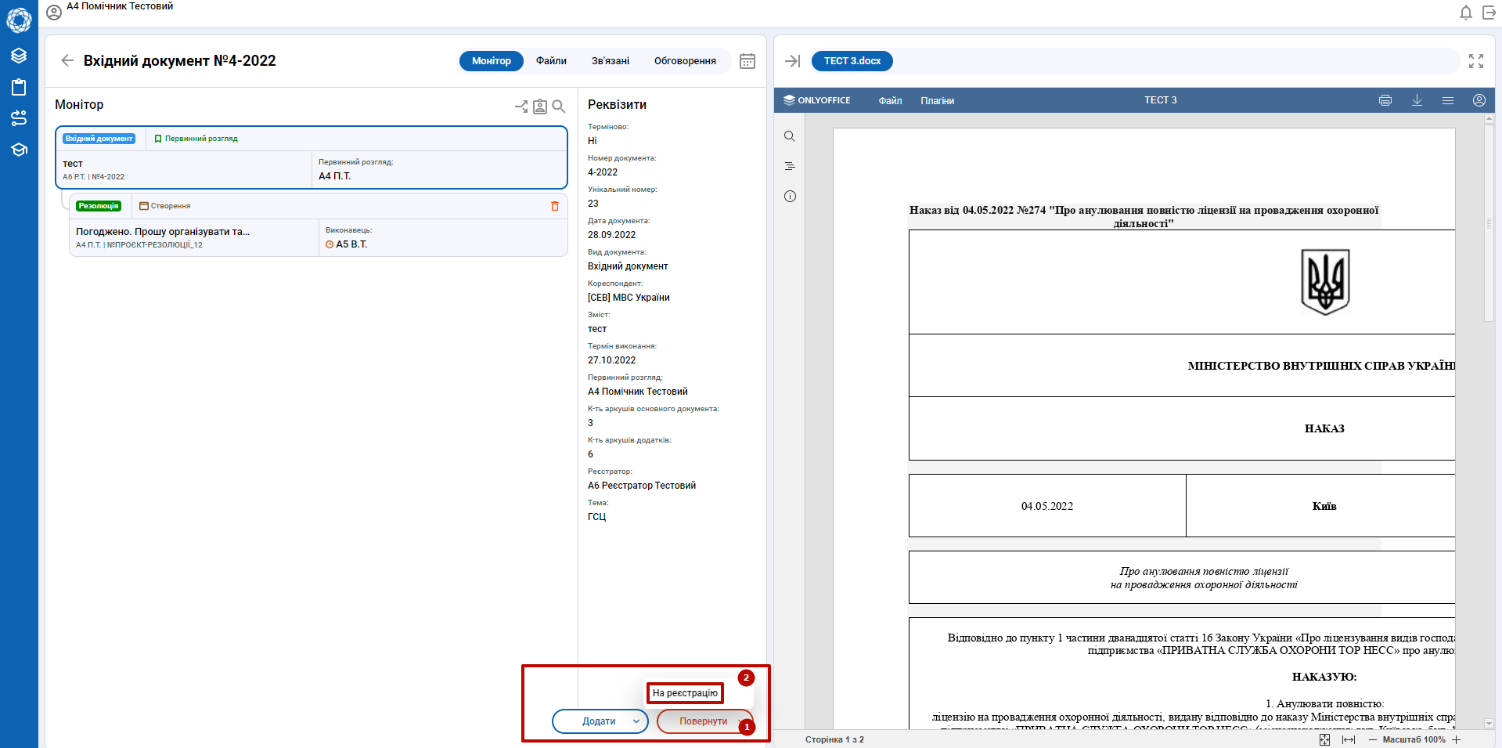
\includegraphics[width=\textwidth]{img/5.2.1.1.png}}
\caption{Рис. 5.2.1.1. }
\end{figure}

--- вкажіть причину повернення → \circled{1} «Змінити особу первинного розгляду» →
натисніть на кнопку, позначену цифрою \circled{2} на Рисунку 5.2.1.2.

\begin{figure}[!htbp]
\centerline{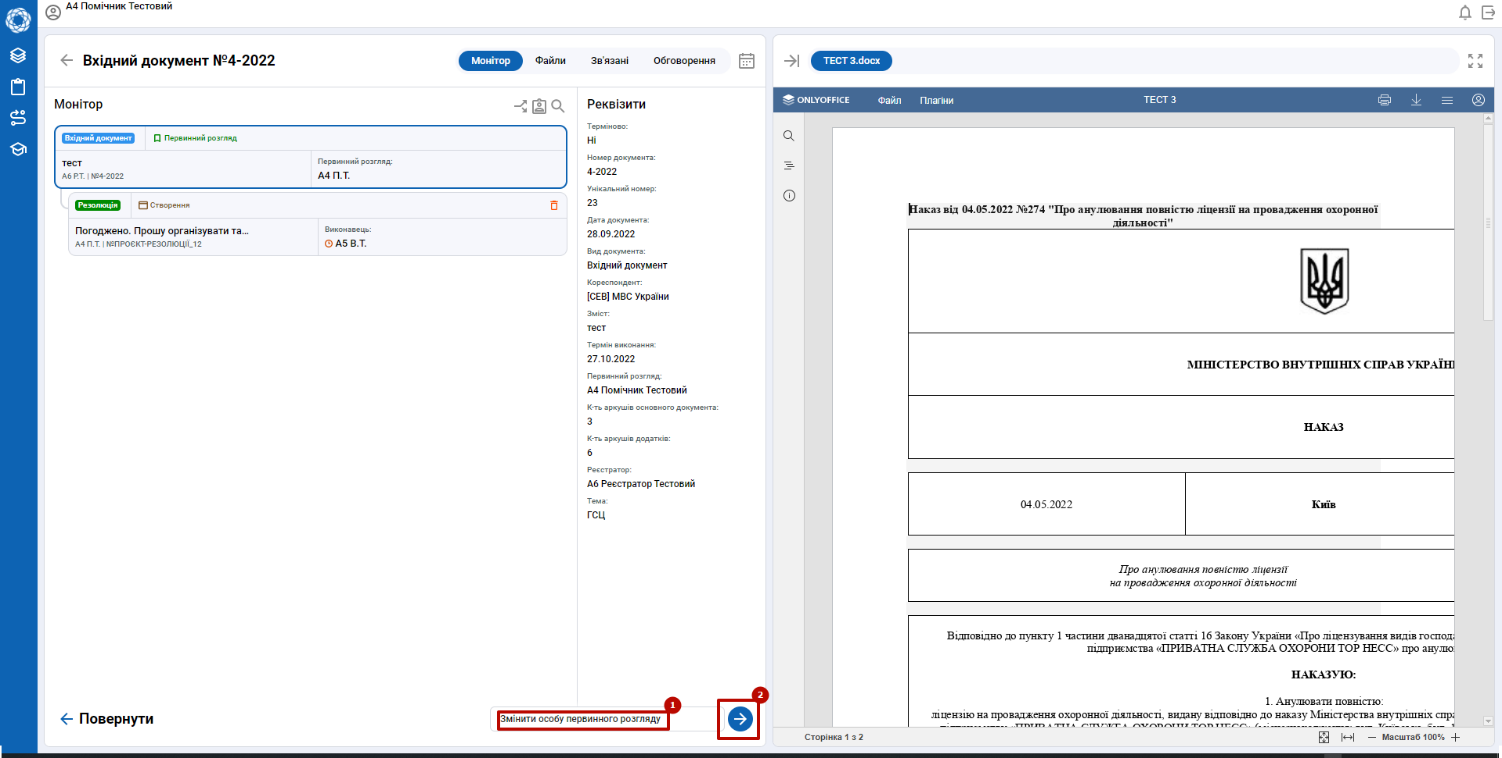
\includegraphics[width=\textwidth]{img/5.2.1.2.png}}
\caption{Рис. 5.2.1.2. Повернення документа на Реєстрацію}
\end{figure}

\subsection{Створення проєкту резолюції}

Для Створення проєкту резолюції помічник/ особа первинного розгляду/ посадова особа, яка отримала резолюцію (завдання):
--- натисніть активний елемент «Додати» → позначено цифрою \circled{1} на Рисунку 5.2.2.1;
--- оберіть пункт «Резолюція» → позначено цифрою \circled{2} на Рисунку 5.2.2.1.

\begin{figure}[!htbp]
\centerline{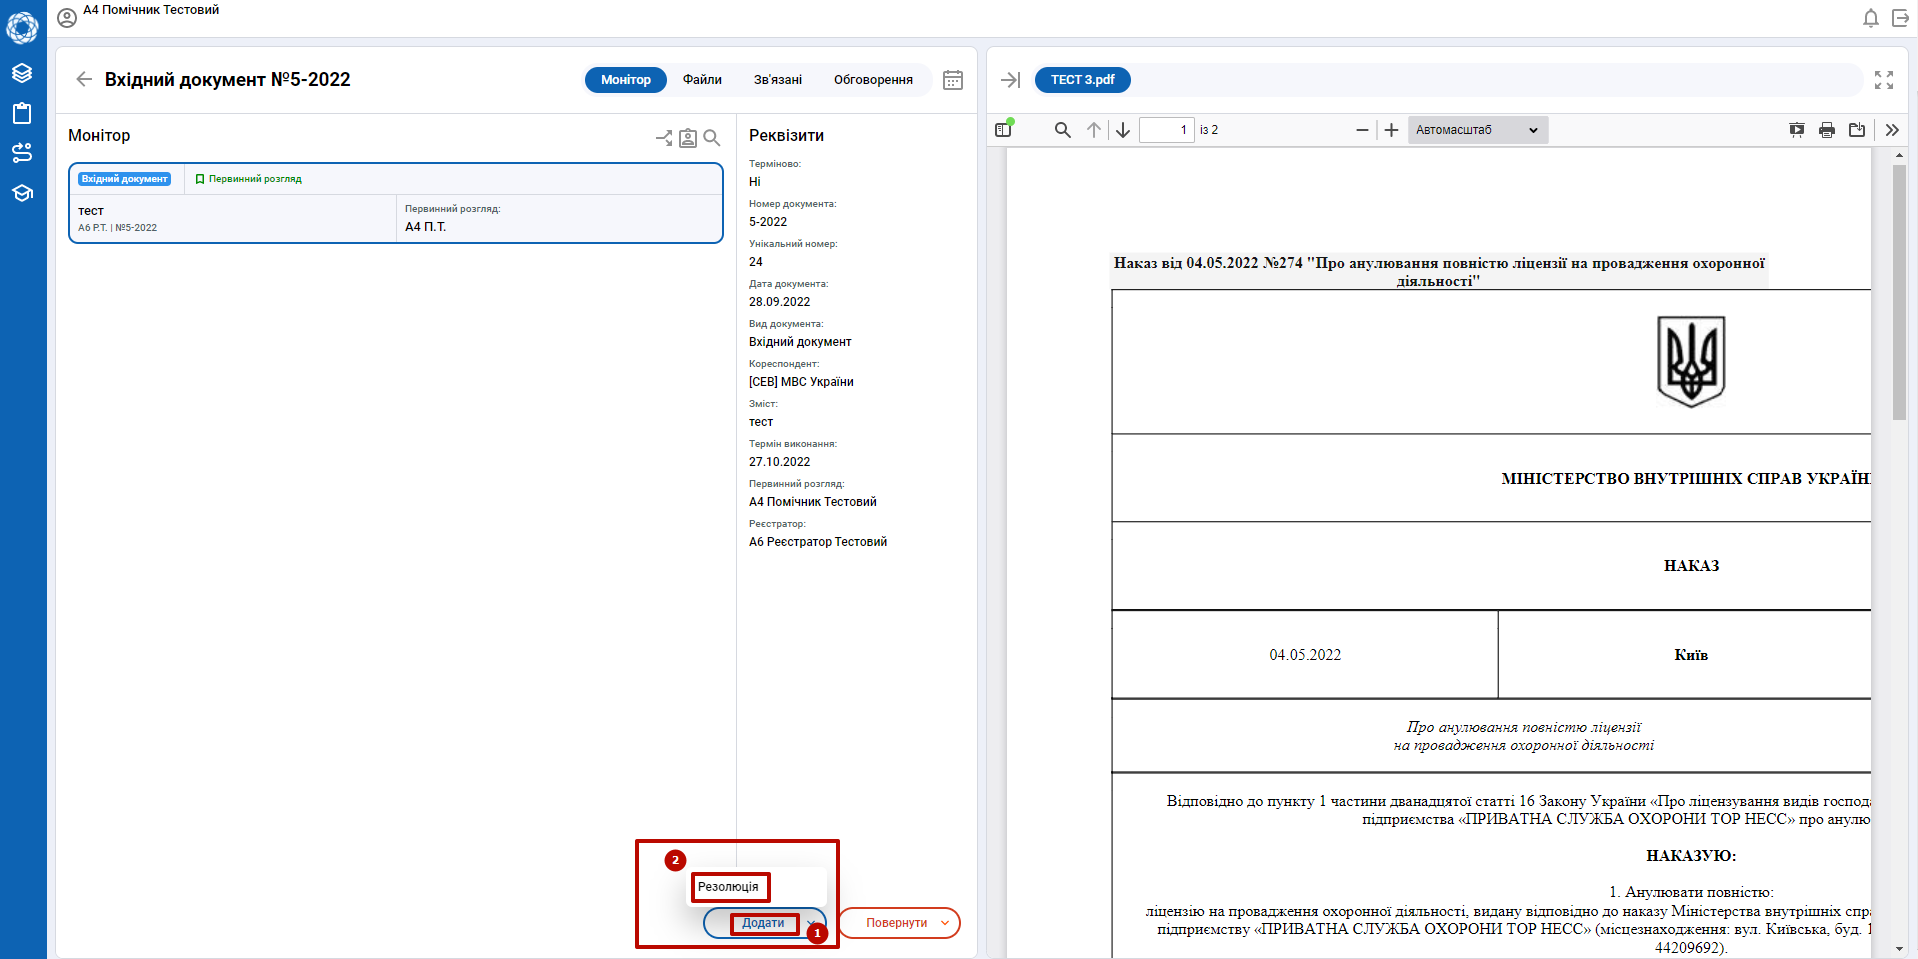
\includegraphics[width=\textwidth]{img/5.2.2.1.png}}
\caption{Рис. 5.2.2.1.}
\end{figure}

введіть реквізити проєкта резолюції в область внесення даних → позначено цифрою \circled{1}
на Рисунку 5.2.2.2 → поля відмічені \circled{$\ast$} – обов'язкові для заповнення;
--- щоб підтвердити → натисніть активний елемент «Створити» → позначено цифрою \circled{2}.

\begin{figure}[!htbp]
\centerline{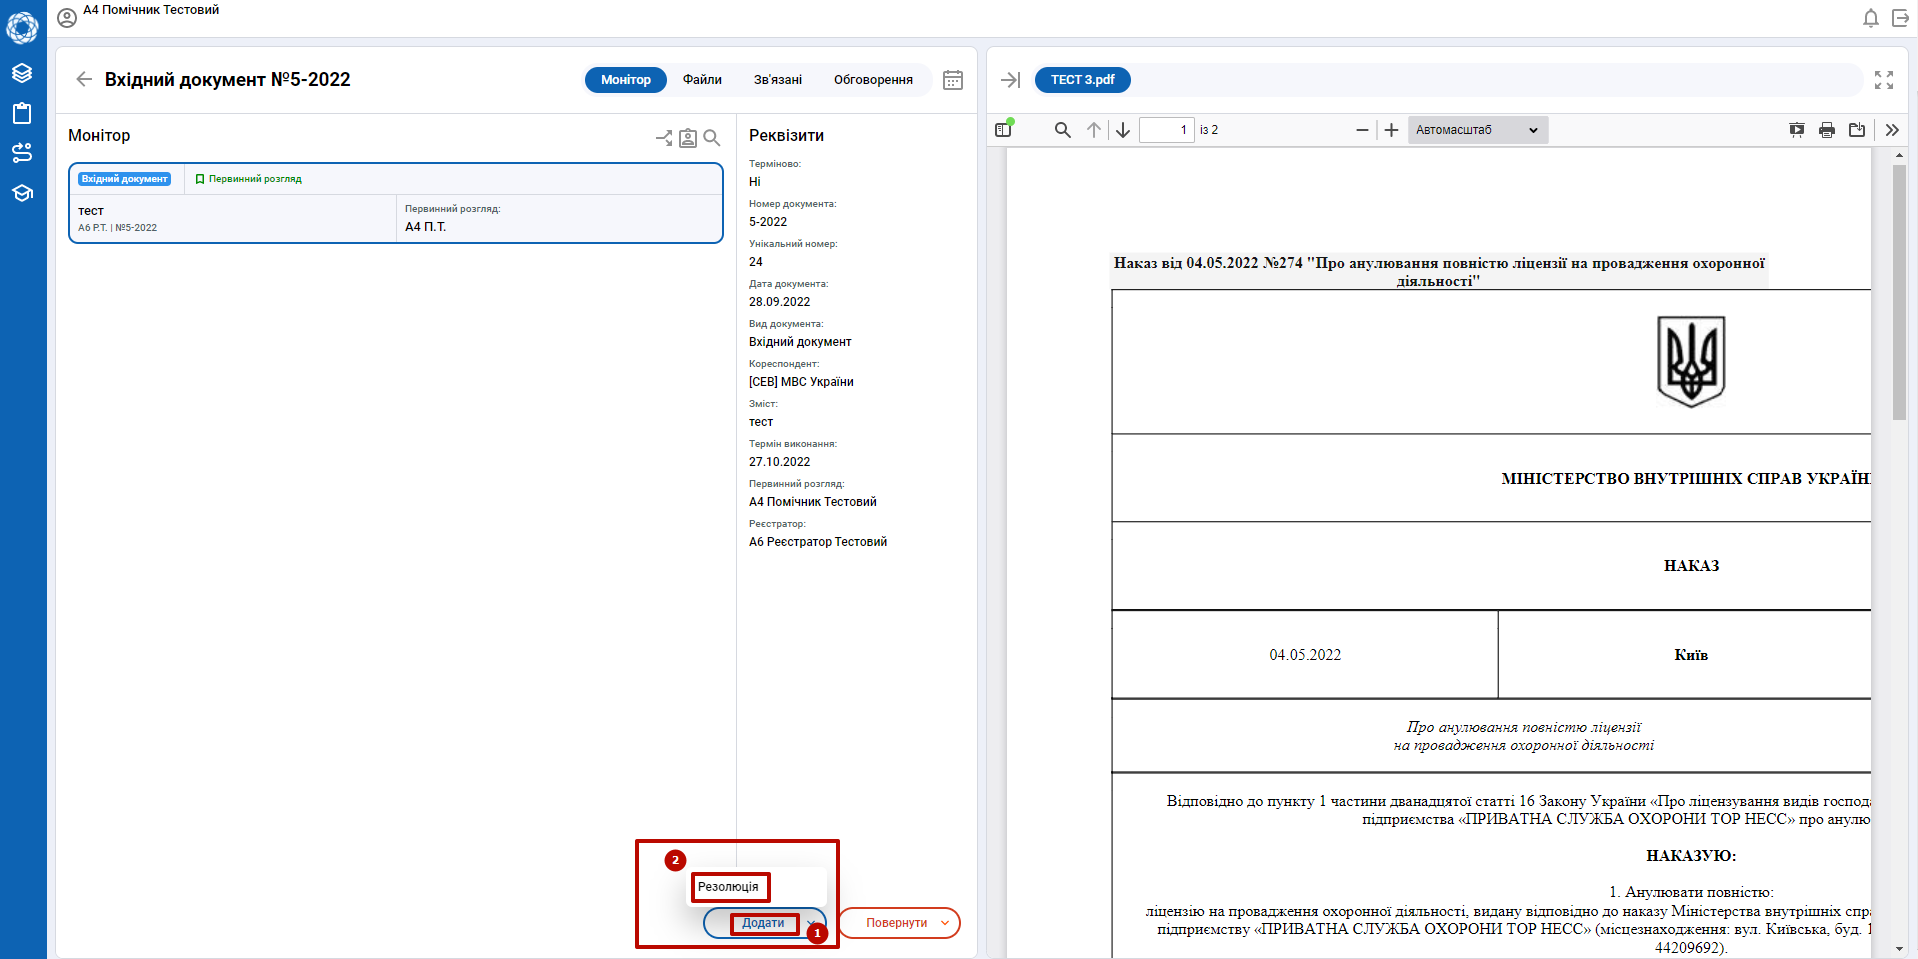
\includegraphics[width=\textwidth]{img/5.2.2.1.png}}
\caption{Рис. 5.2.2.2. Створення проєкту резолюції}
\end{figure}

\subsection{Редагування/видалення проєкту резолюції}

Для Внесення змін у проєкт резолюції:
--- натисніть на піктограму «Редагування» → позначено цифрою \circled{1} на Рисунку 5.2.3.1.

\begin{figure}[!htbp]
\centerline{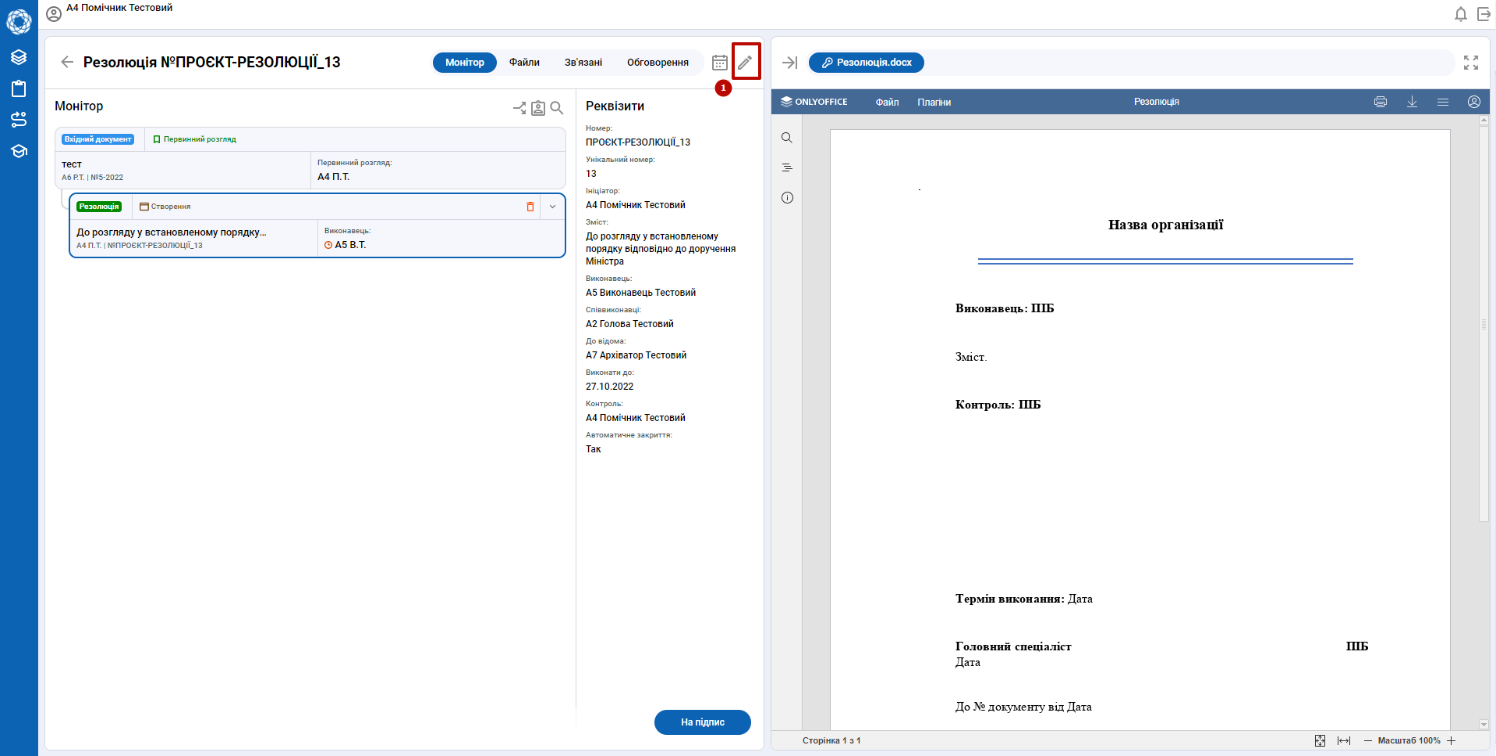
\includegraphics[width=\textwidth]{img/5.2.3.1.png}}
\caption{Рис. 5.2.3.1.}
\end{figure}

--- внесіть необхідні зміни у реквізити документа → для збереження змін
натисніть активний елемент «Змінити» → позначено цифрою \circled{1} на Рисунку 5.2.3.2.

\begin{figure}[!htbp]
\centerline{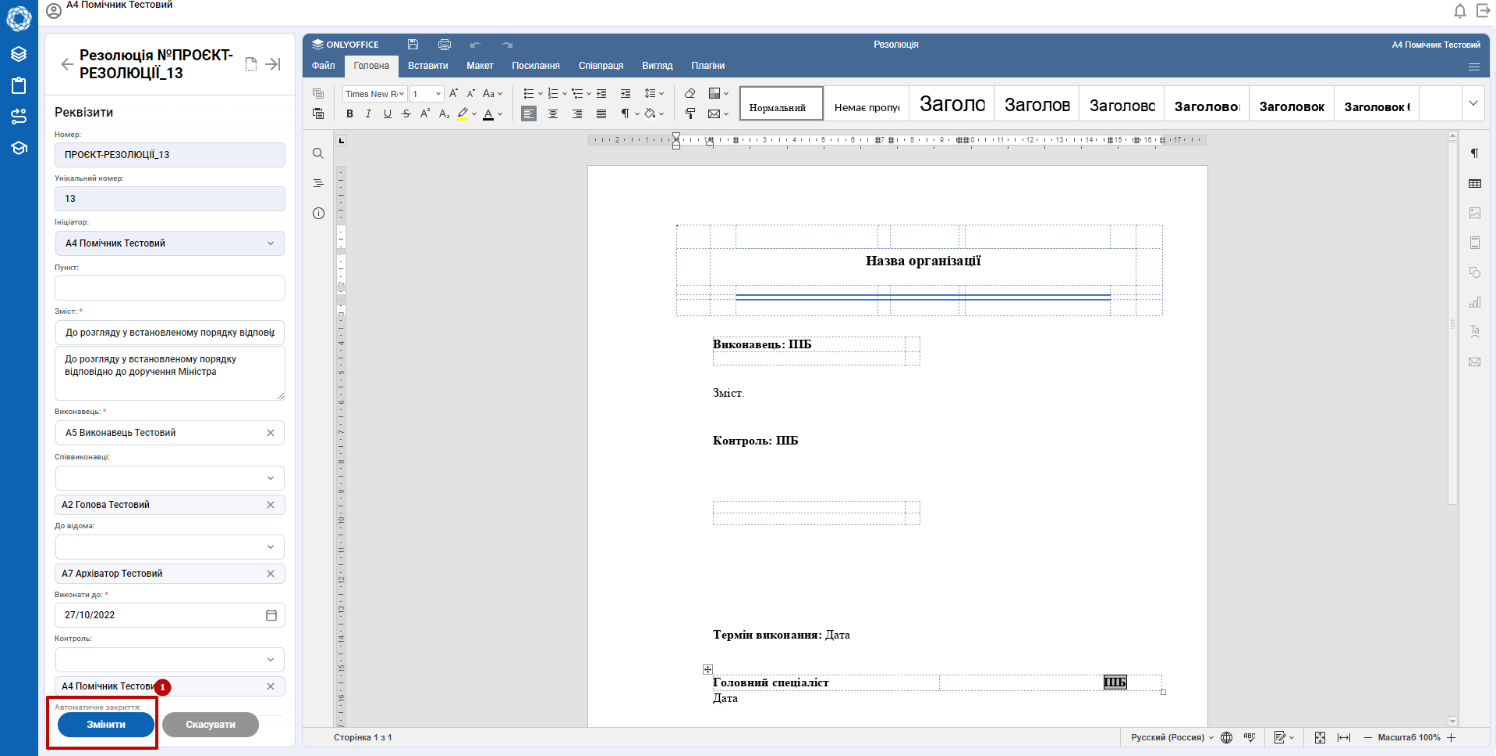
\includegraphics[width=\textwidth]{img/5.2.3.2.png}}
\caption{Рис. 5.2.3.2. Редагування проєкту резолюції}
\end{figure}

Для видалення проєкту резолюції:
--- натисніть піктограму «Видалити» → позначено цифрою \circled{1} на Рисунку 5.2.3.3;
--- розпочніть процес створення резолюції спочатку.

\begin{figure}[!htbp]
\centerline{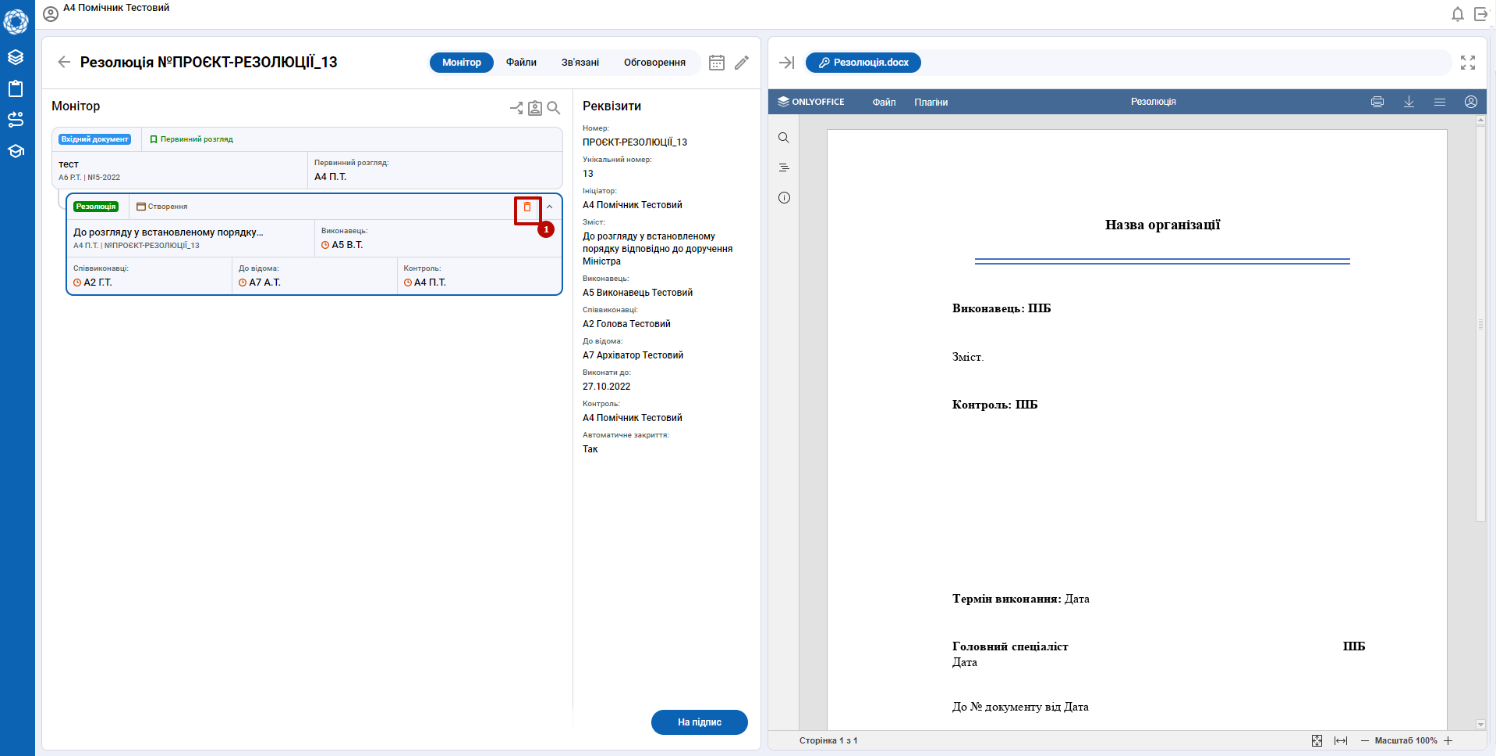
\includegraphics[width=\textwidth]{img/5.2.3.3.png}}
\caption{Рис. 5.2.3.3. Видалення проєкту резолюції}
\end{figure}

\subsection{Підписання проєкту резолюції}

Для Відправлення проєкту резолюції на підписання:
--- натисніть активний елемент «На підпис» → позначено цифрою \circled{1} на Рисунку 5.2.4.1.
--- функція налаштована і доступна керівнику, якому підготовлено проєкт резолюції,
помічнику та особі, що формує проєкт резолюції без помічника.

\begin{figure}[!htbp]
\centerline{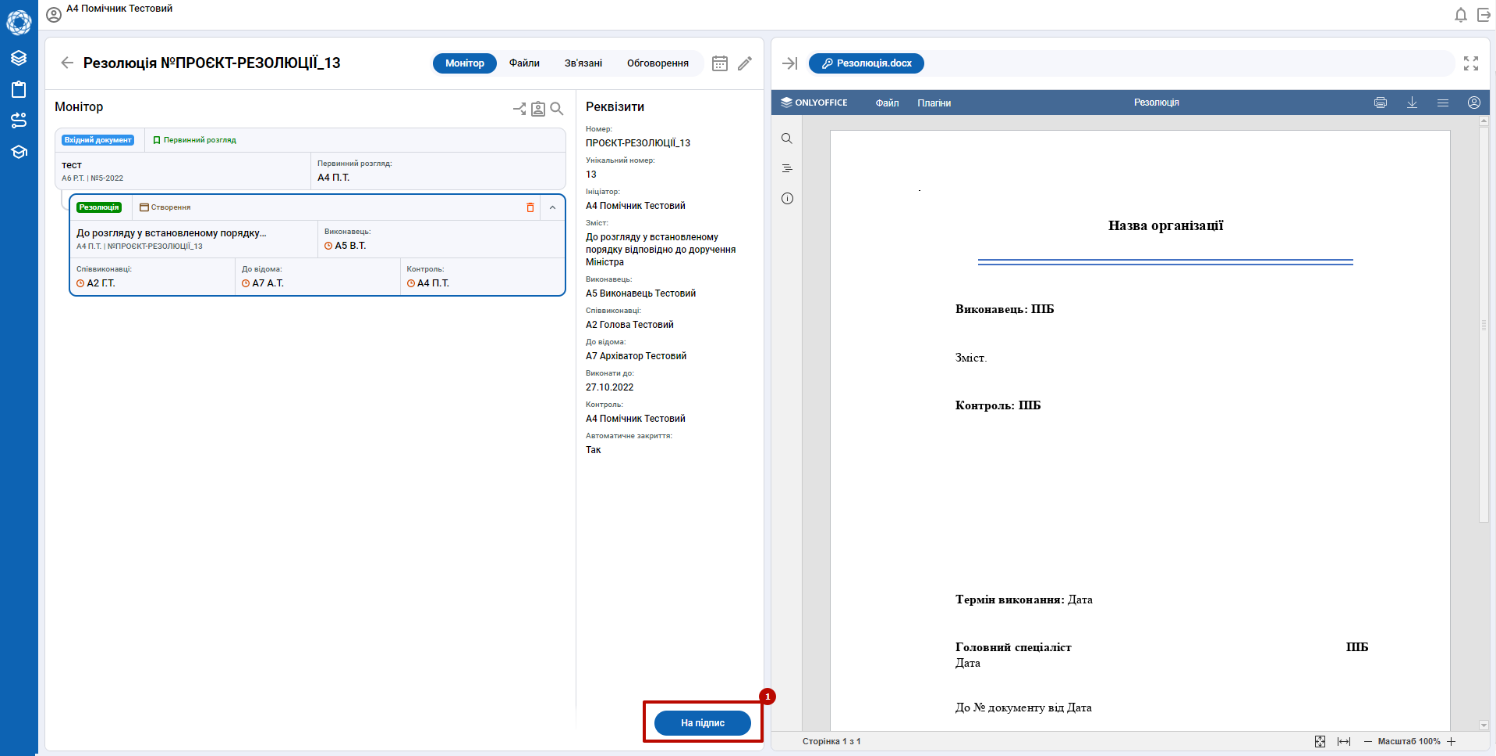
\includegraphics[width=\textwidth]{img/5.2.4.1.png}}
\caption{Рис. 5.2.4.1. }
\end{figure}

Для підпису проєкту резолюції:
--- натисніть активний елемент «Підписати» → позначено цифрою \circled{1} на Рисунку 5.2.4.2.
Для повернення проєкту резолюції на Створення:
--- натисніть активний елемент «Повернути» → позначено цифрою \circled{2} →
виберіть пункт «На створення» → позначено цифрою \circled{3} на Рисунку 5.2.4.2.

\begin{figure}[!htbp]
\centerline{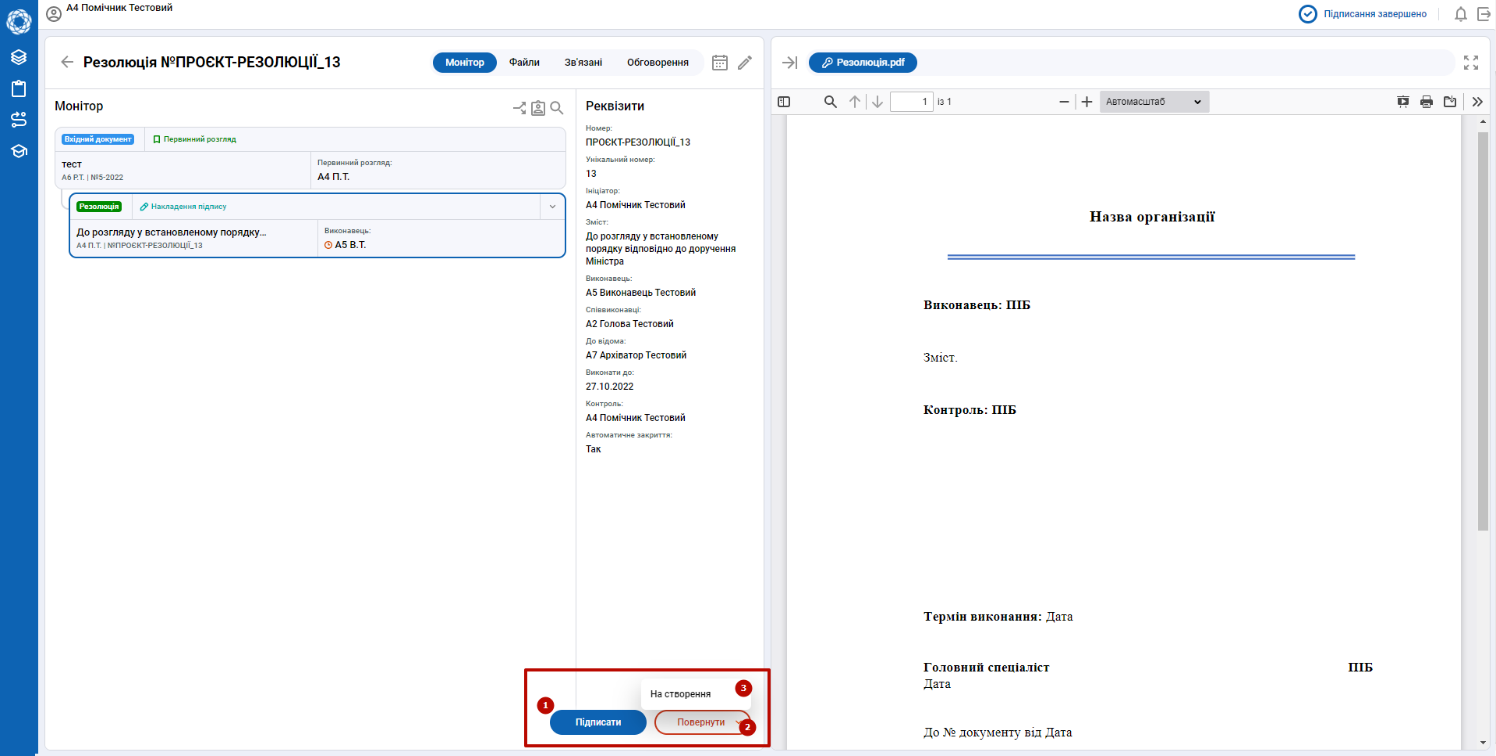
\includegraphics[width=\textwidth]{img/5.2.4.2.png}}
\caption{Рис. 5.2.4.2. }
\end{figure}

\subsection{Виконання/відхилення резолюції}

Резолюція стосовно виконання вхідного документа може передбачати проведення
виконавцем певних дій (підготувати документ) або бути нейтральною, наприклад
«взято до відома». В усіх випадках необхідно підтвердити Виконання:
--- натисніть активний елемент «Виконано» → позначено цифрою \circled{1} на Рисунку 5.2.5.1;
--- обов'язково зазначте результат опрацювання на вкладці «Обговорення» →
позначено цифрою \circled{2} на Рисунку 5.2.5.1.

\section{Вихідний документ}

\begin{figure}[!htbp]
\centerline{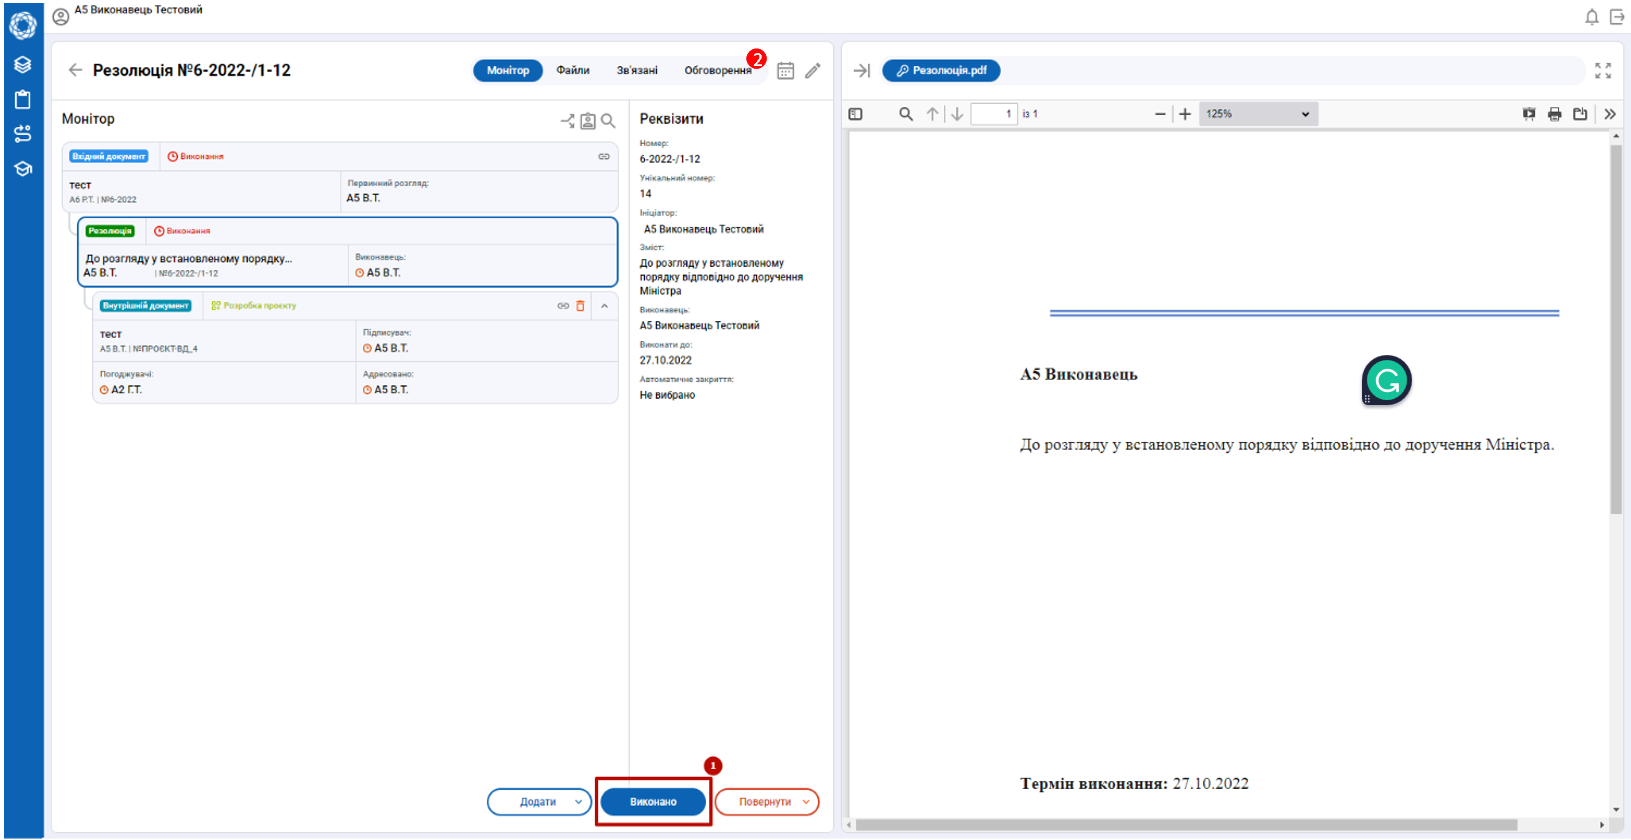
\includegraphics[width=\textwidth]{img/5.2.5.1.png}}
\caption{Рис. 5.2.5.1. Підтвердження виконання листа}
\end{figure}

щоб скористатися підменю вкладки «Обговорення» → натисніть на цю
вкладку, що позначена цифрою \circled{2} на Рисунку 5.2.5.1 → з'явиться нова
форма екранного меню, що містить поля для введення інформації та
коментарів → як це показано на Рисунку 5.2.5.2.

Цифрами на Рисунку 5.2.5.2 позначено:
\circled{1} --- поточна вкладка;
\circled{2} --- поле для введення тесту з вказанням результату опрацювання документа;
\circled{3} --- поле для коментарів.

\begin{figure}[!htbp]
\centerline{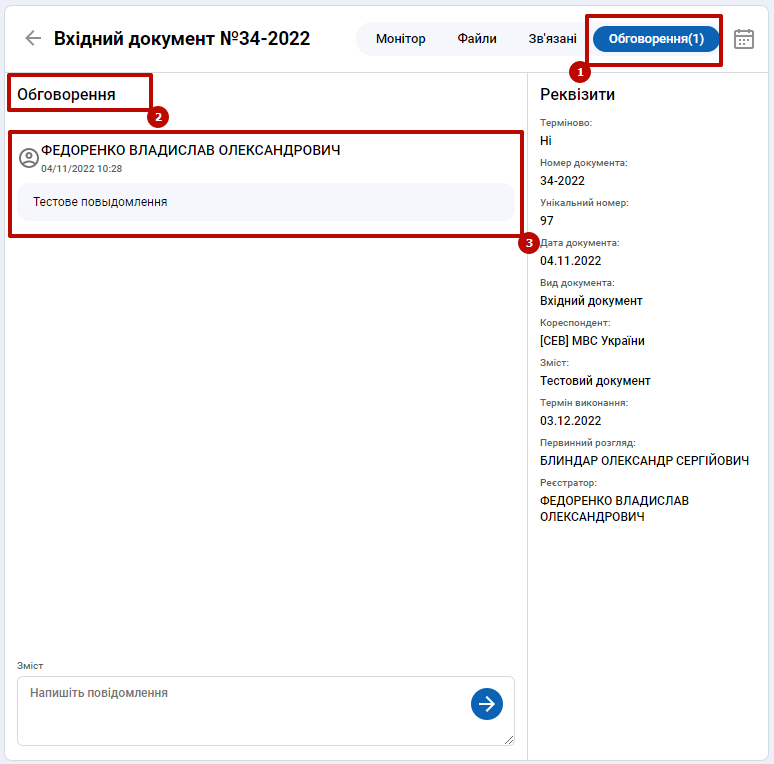
\includegraphics[width=\textwidth]{img/5.2.5.2.png}}
\caption{Рис. 5.2.5.2. Результат опрацювання документа}
\end{figure}

В процесі розгляду вхідного документа виконавцем, може з'ясуватися, що
призначене завдання знаходиться поза межами його компетенції, у такому разі
документ повертають на попередню стадію:
--- натисніть активний елемент «Повернути» → позначено цифрою \circled{1} на Рисунку 5.2.5.3;
--- обрати пункт «На попередню стадію» → позначено цифрою \circled{2} на Рисунку 5.2.5.3.

\begin{figure}[!htbp]
\centerline{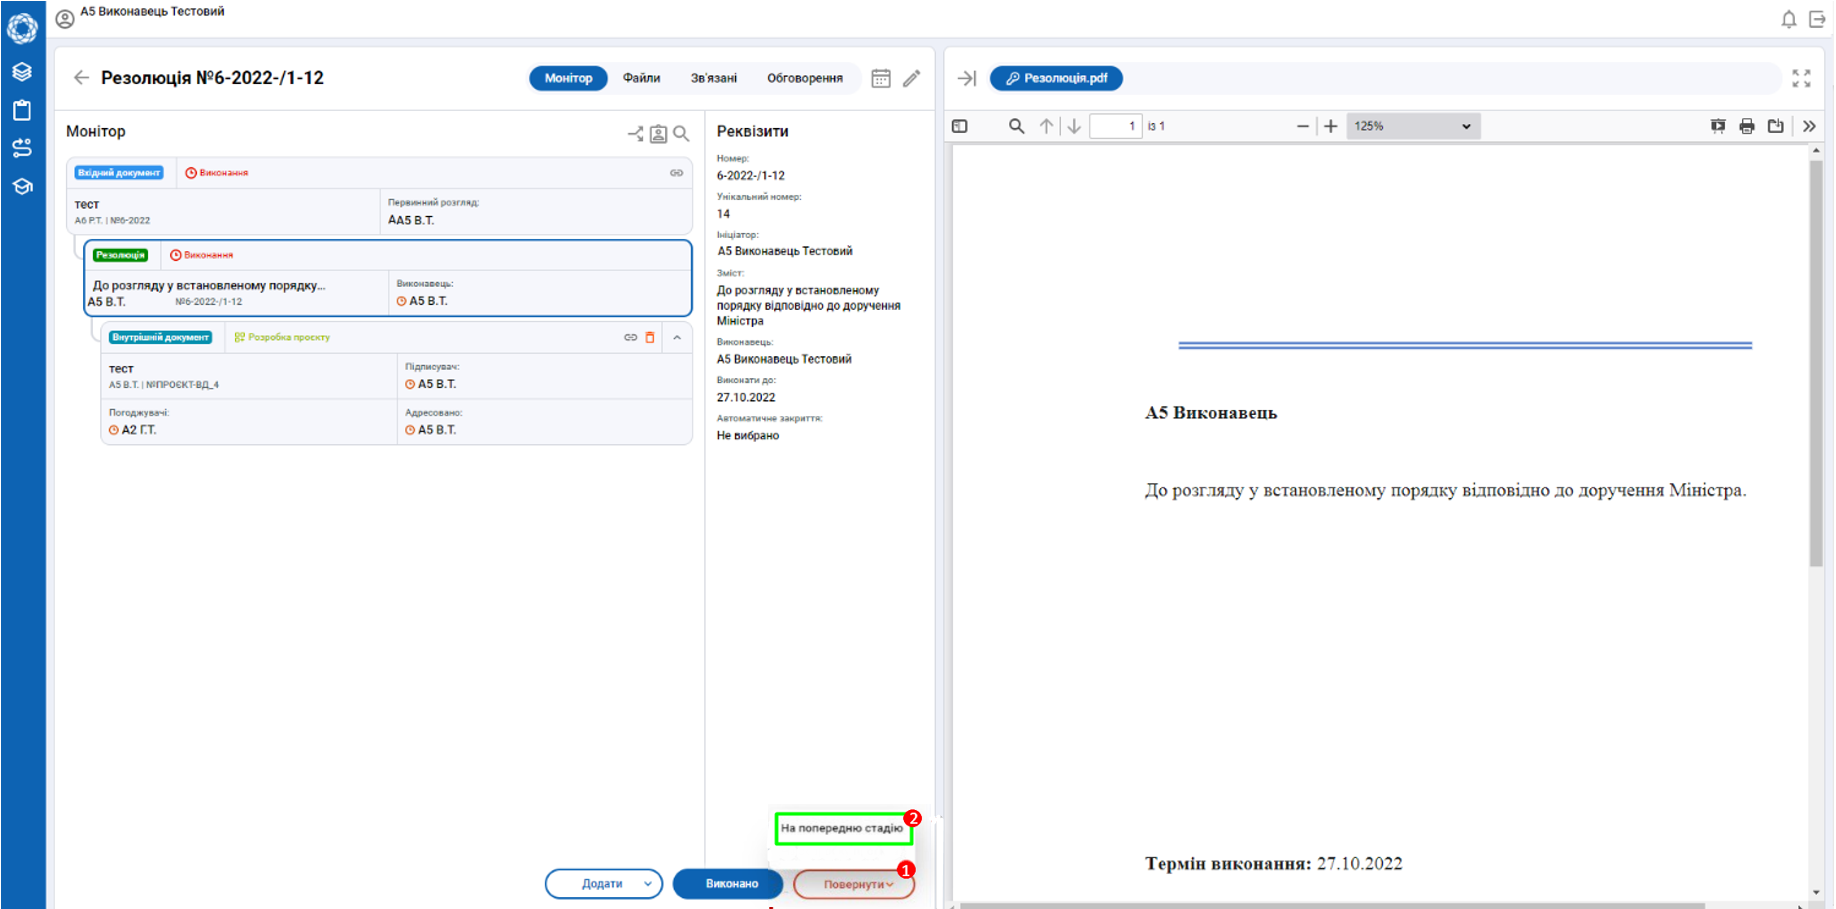
\includegraphics[width=\textwidth]{img/5.2.5.3.png}}
\caption{Рис. 5.2.5.3. Повернення документа на попередню стадію}
\end{figure}

Обов'язково вкажіть причину повернення документа:
--- «Змінити виконавця документа» → позначено цифрою \circled{1} на Рисунку 5.2.5.4
→ натисніть елемент \circled{→} → позначено цифрою \circled{2} на Рисунку 5.2.5.4.

\begin{figure}[!htbp]
\centerline{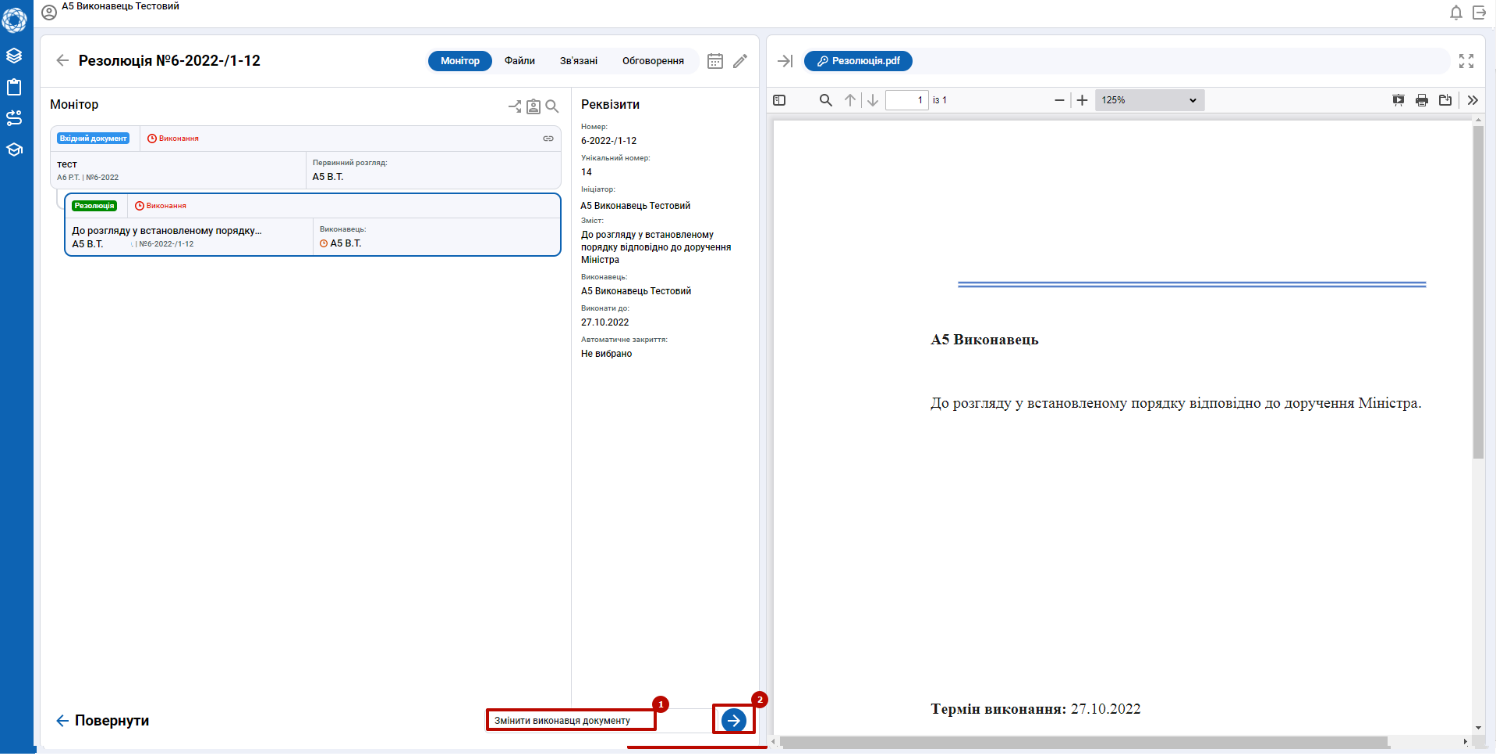
\includegraphics[width=\textwidth]{img/5.2.5.4.png}}
\caption{Рис. 5.2.5.4. Причина повернення документа}
\end{figure}

\subsection{Створення проєкту вихідного документу \\ на основі резолюції}

Для Створення проєкту вихідного документа:
--- натисніть активний елемент «Додати» → позначено цифрою \circled{1} на Рисунку 5.3.1.1;
--- \circled{→} виберіть з розгорнутого переліку «Вихідний документ» → позначено цифрою \circled{2} на Рисунку 5.3.1.1.

\begin{figure}[!htbp]
\centerline{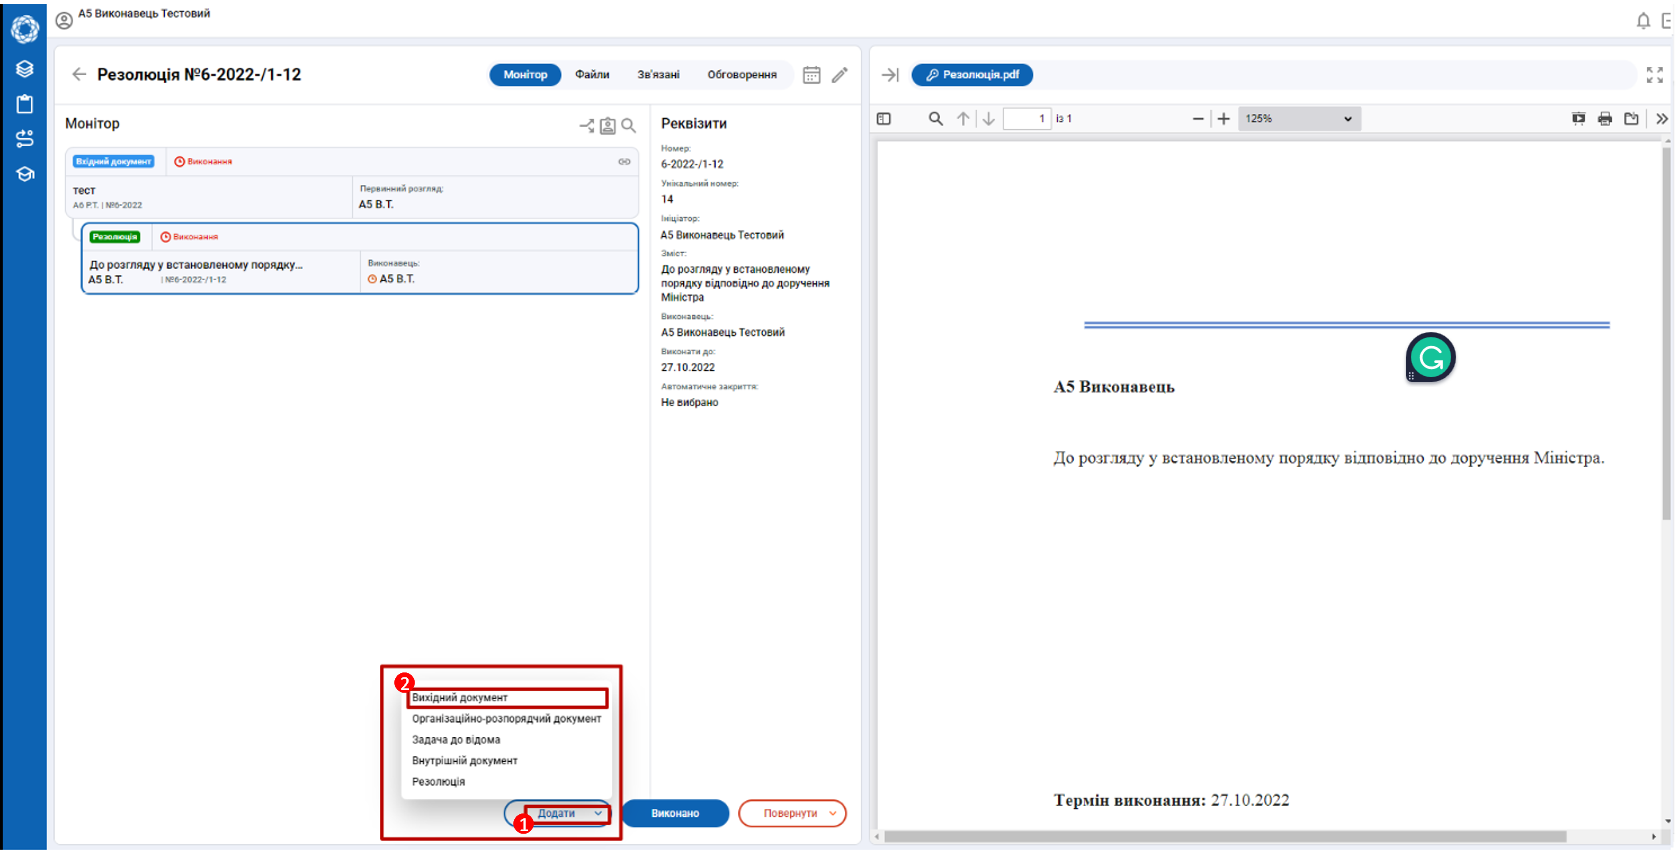
\includegraphics[width=\textwidth]{img/5.3.1.1.png}}
\caption{Рис. 5.3.1.1. Етапи створення проєкту вихідного документа}
\end{figure}

на екрані за замовчуванням відкриється підменю «Вихідний документ» →
позначено цифрою 1 на Рисунку 5.3.1.2, що являє собою область для введення даних РМК;
--- виберіть вид документа «Вихідний лист» → позначено цифрою \circled{2} на Рисунку 5.3.1.2;
--- заповніть РМК в області введення даних → позначена цифрою \circled{3} (виділена рамкою) на Рисунку 5.3.1.2;
--- важливо: поля відмічені \circled{$\ast$} обов’язкові для заповнення.

\begin{figure}[!htbp]
\centerline{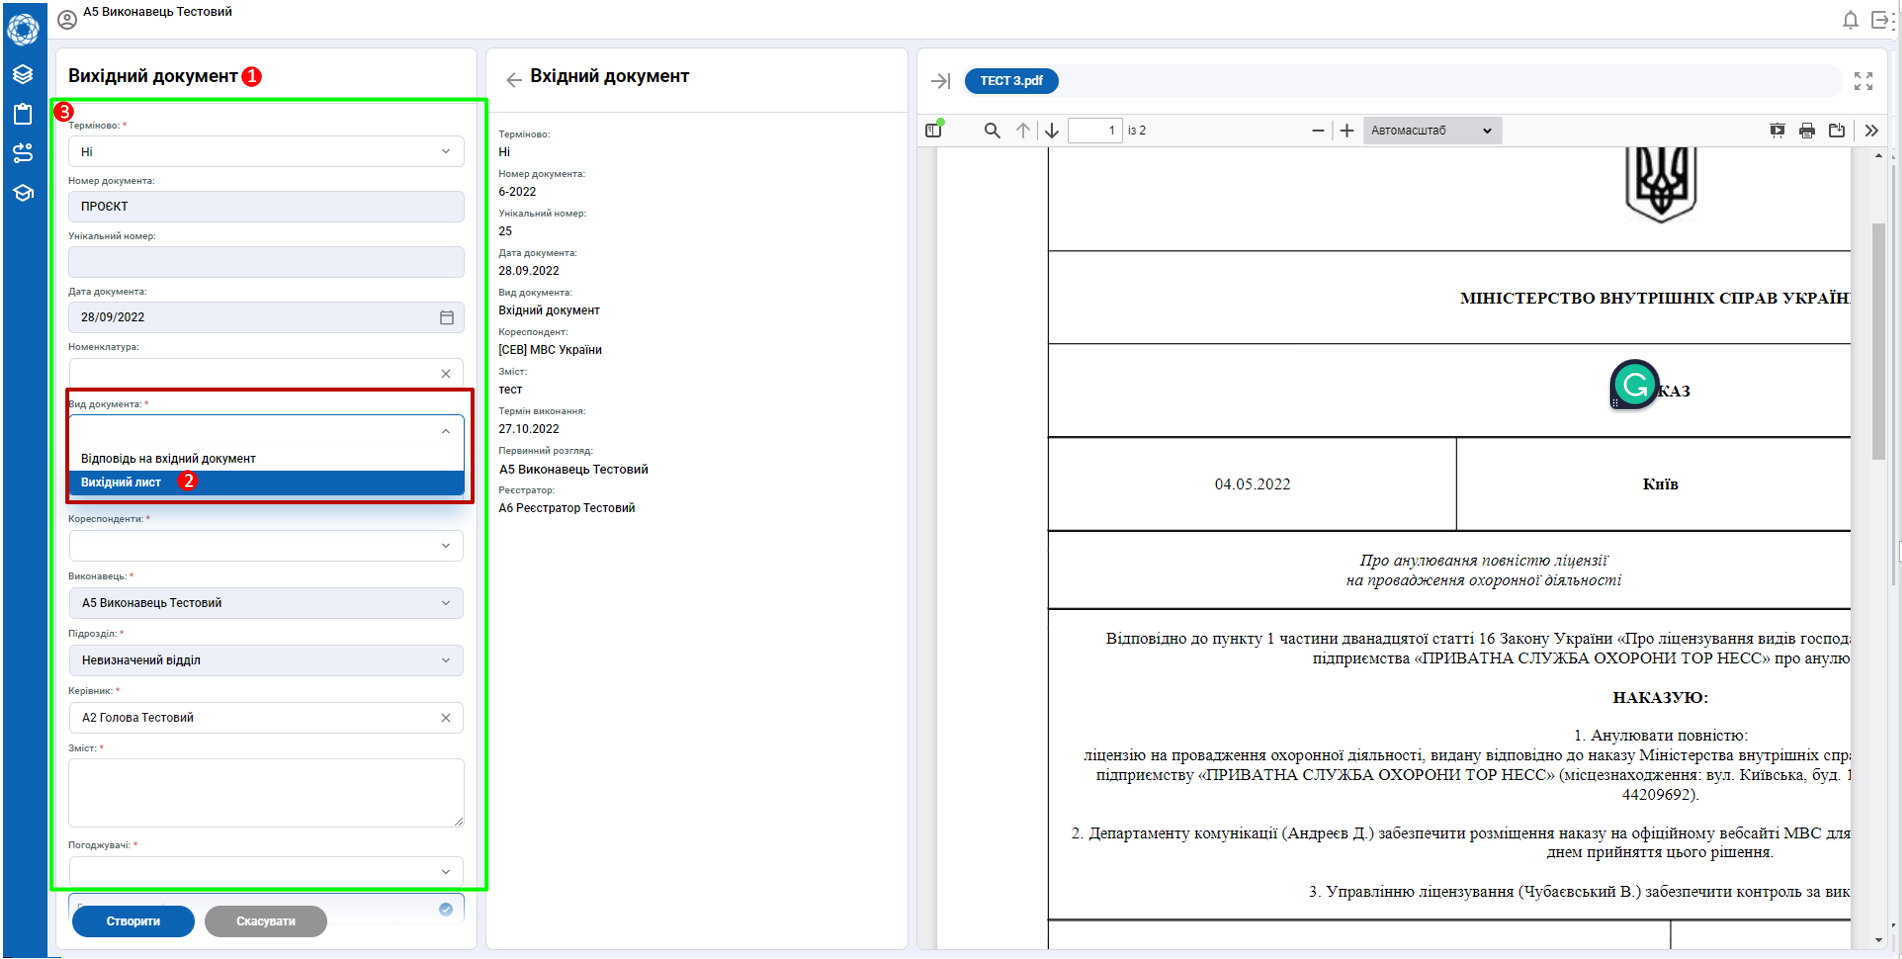
\includegraphics[width=\textwidth]{img/5.3.1.2.png}}
\caption{Рис. 5.3.1.2. Етапи створення проєкту вихідного документа}
\end{figure}

оберіть тип шаблону «Порожній вихідний документ» → позначено цифрою \circled{1} (виділено рамкою) на Рисунку 5.3.1.3;
--- натисніть активний елемент «Створити» → позначено цифрою \circled{2} на Рисунку 5.3.1.3;
--- вихідний документ успішно створено.

\begin{figure}[!htbp]
\centerline{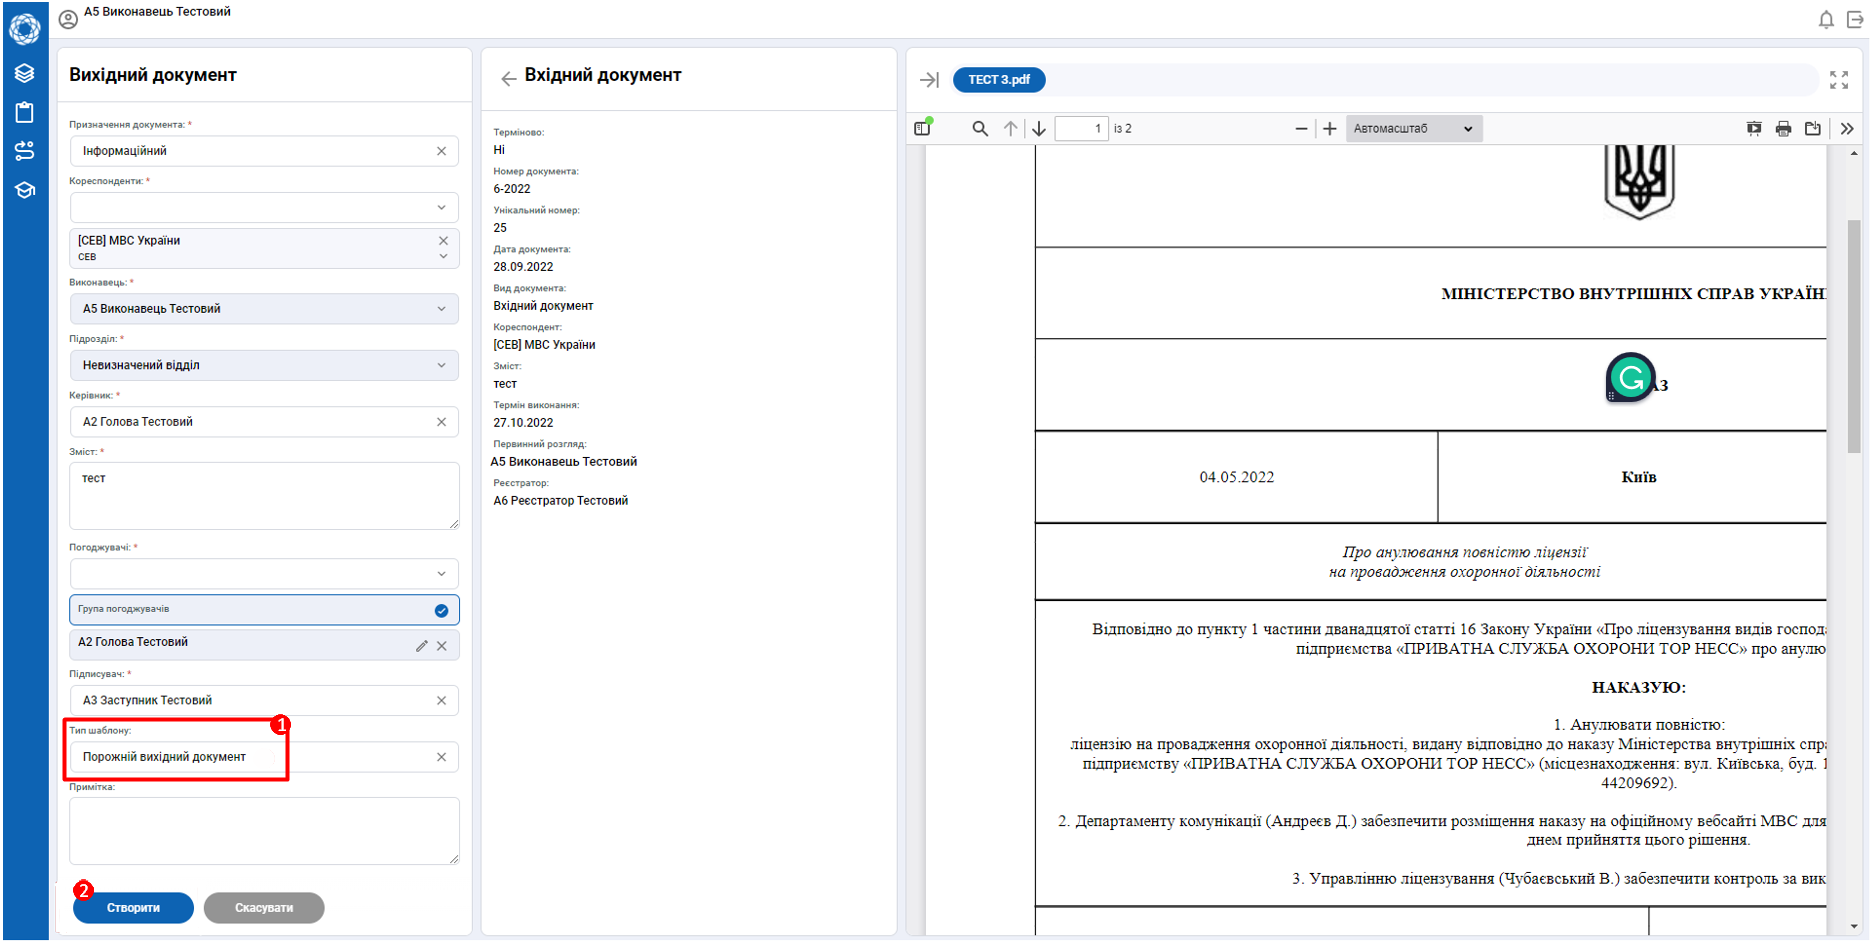
\includegraphics[width=\textwidth]{img/5.3.1.3.png}}
\caption{Рис. 5.3.1.3. Створення проєкту вихідного документа}
\end{figure}

\subsection{Редагування вихідного документу}

Після створення на попередньому етапі вихідного документа, існує
можливість змінити попередньо внесені дані (у разі необхідності) за допомогою
редагування.

Для Редагування вихідного документа:
--- відкрити меню редагування (піктограма із зображенням олівця у верхній лівій частині екранної форми);
--- користувач має змогу внести зміни наступного характеру:
1) виправити/ змінити дані в РМК → область позначена цифрою \circled{1} на Рисунку 5.3.2.1;
2) додати матеріали → (перетягнути файл/ натиснути щоб додати файл) в поле, позначене цифрою \circled{2} на Рисунку 5.3.2.1;
3) додати відскановані документи → позначено цифрою \circled{3} на Рисунку 5.3.2.1 (функціональність піктограми сканування описано в пункті 5.1.2 розділу 5);
4) заповнити шаблон/ відредагувати доданий файл (якщо він у форматі $\ast$.docx) → область позначена цифрою \circled{4} на Рисунку 5.3.2.1;
5) після внесення відповідних змін → натисніть піктограму «Зберегти» → позначено цифрою \circled{5} на Рисунку 5.3.2.1.

\begin{figure}[!htbp]
\centerline{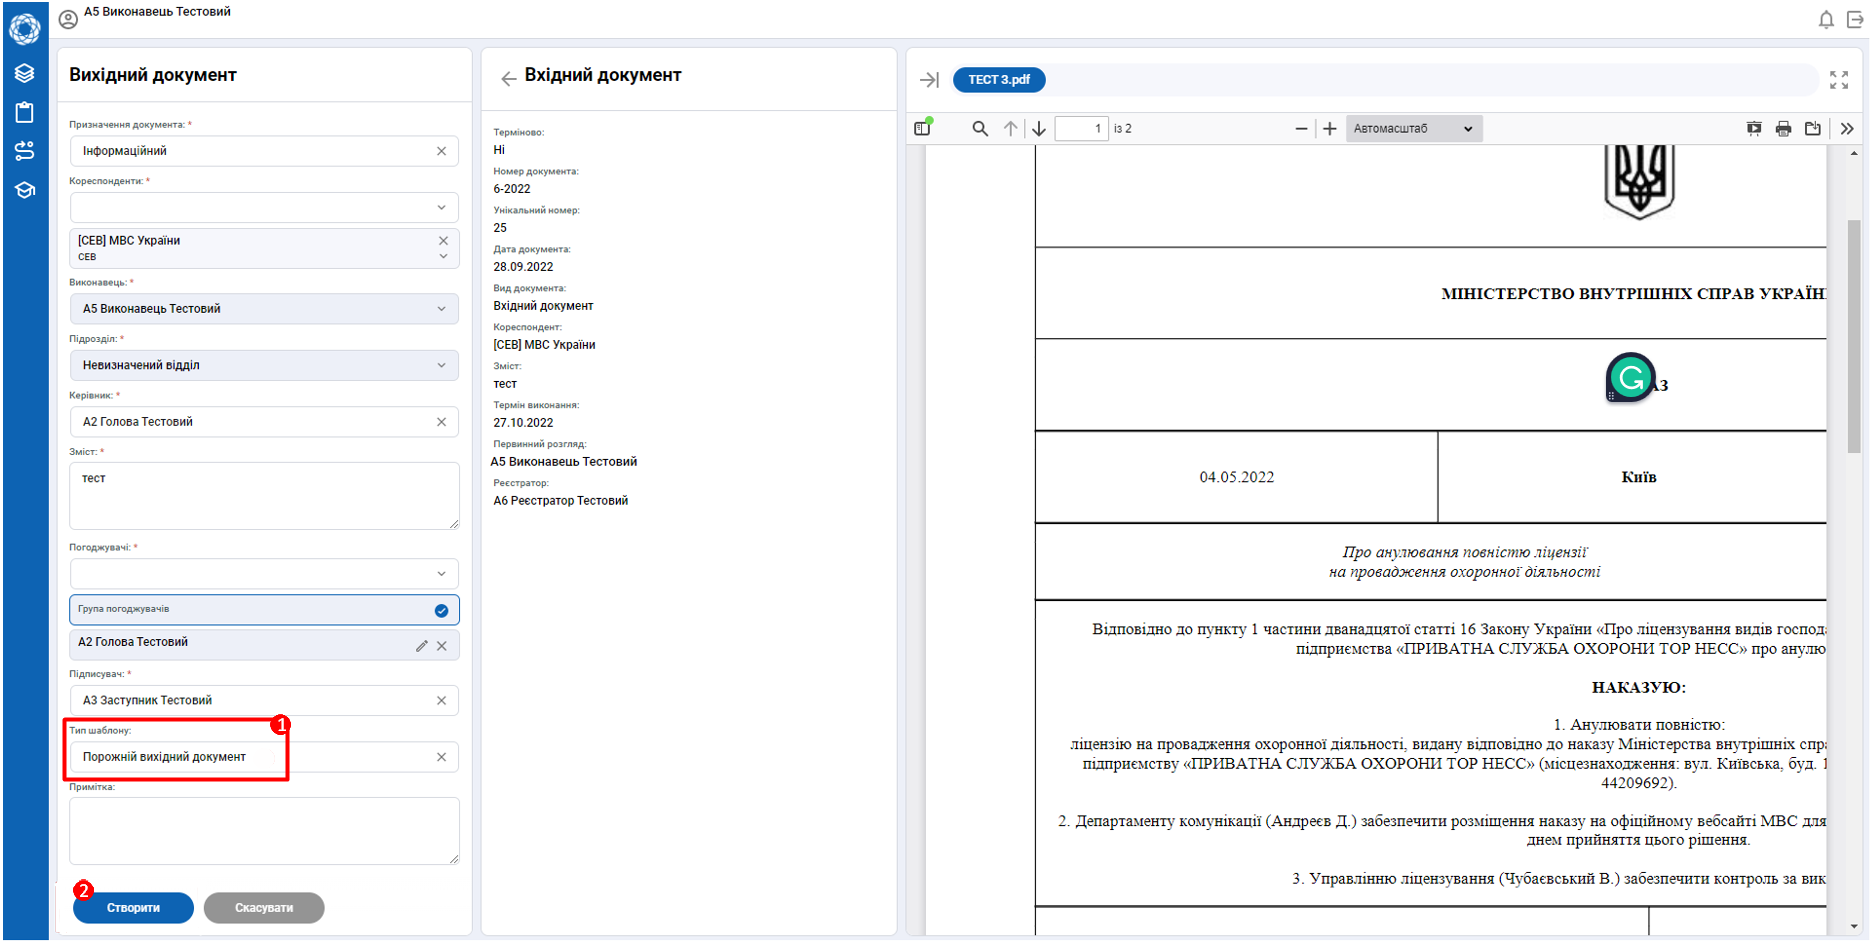
\includegraphics[width=\textwidth]{img/5.3.1.3.png}}
\caption{Рис. 5.3.2.1. Процес внесення змін у документ}
\end{figure}

щоб підтвердити введення змін → натисніть активний елемент «Змінити» → позначено червоною рамкою на Рисунку 5.3.2.2

\begin{figure}[!htbp]
\centerline{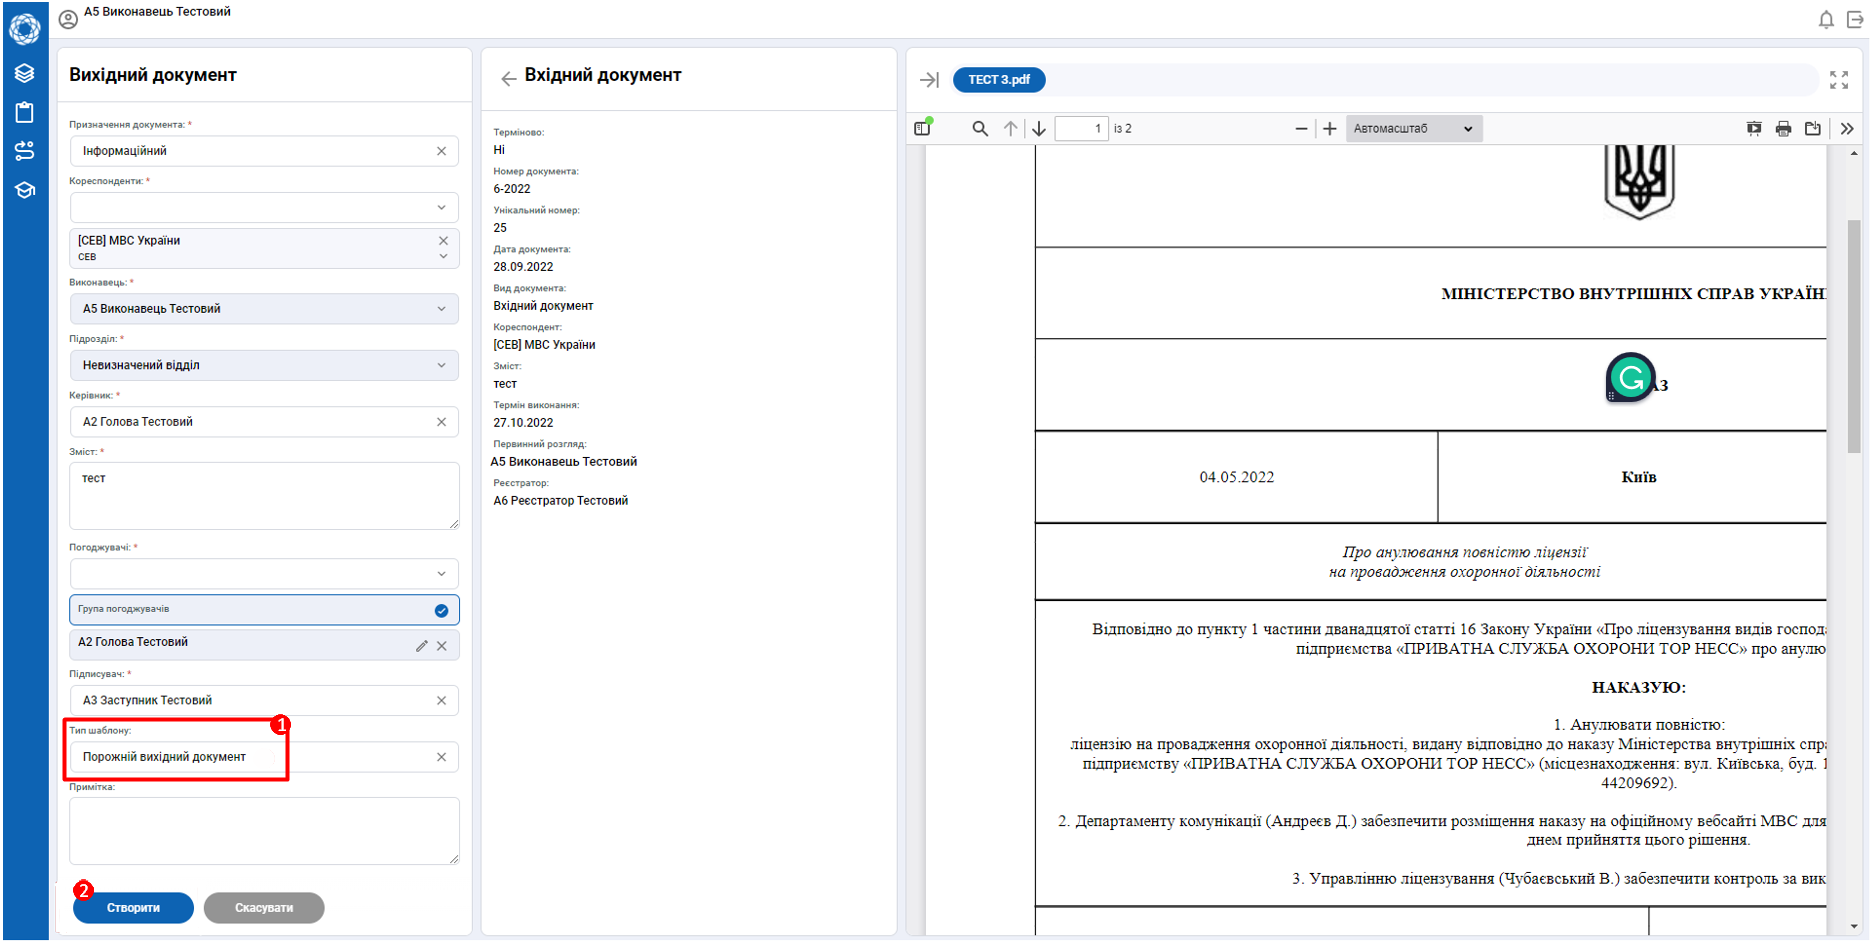
\includegraphics[width=\textwidth]{img/5.3.1.3.png}}
\caption{Рис. 5.3.2.2. Завершальний етап внесення змін у документ}
\end{figure}

\subsection{Видалення проєкту вихідного документа}

\section{Внутрішній документ}

\subsection{Створення проєкту \\ внутрішнього документа \\ на основі резолюції}

\subsection{Редагування проєкту \\ внутрішнього документу \\ на основі резолюції}

\subsection{Видалення проєкту \\ внутрішнього документу \\ на основі резолюції}

\section{Організаційно-розпорядчі документи}

\subsection{Створення проєкта \\ організаційно-розпорядчого документа}

\subsection{Редагування \\ організаційно-розпорядчого документа}

\subsection{Видалення проєкта \\ організаційно-розпорядчого документа}

\section{Пошук документів}

\section{Погодження проєкту документа}

\subsection{Редагування проєкту документа}

\subsection{Повернення проєкта документа}

\section{Групування}

\section{Проєкт відправки}

